\documentclass[fontsize=12pt,paper=letter,overfullrule=yes]{scrbook}

% for 1.5 line spacing
\usepackage{setspace}
\onehalfspacing
% single spacing for table of contents
\AfterTOCHead{\singlespacing}

% recompute page layout based on the above
\recalctypearea

% more colors (like RedOrange)
\usepackage[dvipsnames]{xcolor}

% qualitative colors
% subset of https://jfly.uni-koeln.de/color/
% that is also distinctive in grayscale
\definecolor{set1}{HTML}{0071b2} % blue
\definecolor{set2}{HTML}{e59c00} % orange
\definecolor{set3}{HTML}{009e73} % green
\definecolor{set4}{HTML}{efe440} % yellow

% so we can splice in PDFs
\usepackage{pdfpages}

% set up bibliography
\usepackage[
  backend=bibtex,
  sortcites=true,
  sorting=ynt,
  abbreviate=false,
  style=numeric,
  citestyle=numeric,
  isbn=false,
  url=false,
  doi=false]{biblatex}
\addbibresource{bibliography.bib}

% enumerate* and itemize*
\usepackage[inline]{enumitem}

% for \begin{comment}
\usepackage{verbatim}

% for source-code listings
\usepackage[newfloat,draft=false]{minted}

% for formulas
\usepackage{mathtools}

% to split lists into multiple columns
\usepackage{multicol}

% for "on page NN" reference
\usepackage[nospace]{varioref}

% for \sfrac
\usepackage{xfrac}

% for \ifoptionfinal
\usepackage{ifdraft}

% do not reset page numbers at \mainmatter
\let\mainmatterorig\mainmatter
\renewcommand\mainmatter
 {\edef\p{\arabic{page}}%
  \mainmatterorig
  % we need to compute the actual current page number. we know the page number
  % from _before_ we called \mainmatter. but what is it now? well, it is
  % certainly that +1. but we also need to account for the next chapter starting
  % on a "right" (odd) page. we do this by adding the page number modulo two.
  % TODO: double check before final version
  \setcounter{page}{\p+1+(\p-\p/2*2)}%
 }

% an environment for todos
\newenvironment{inprogress}
  {\vspace{.5em} \color{set2} \noindent \textbf{TODO}}
  {\vspace{.5em}}

% a command to indicate current editing progress
\newcommand{\resume}{
  \begin{center}
    \color{set2}
    \hrule
    \vspace{1pt}
    \hrule
    \hrule
    \vspace{10pt}
    \textbf{This section is not yet complete.}
    \vspace{10pt}
    \hrule
    \hrule
    \vspace{1pt}
    \hrule
  \end{center}
}

% an environment for invariants
\newcounter{invn}
\renewcommand{\theinvn}{\Roman{invn}}
\newenvironment{invariant}
  {\vspace{.5em} \color{set1} \refstepcounter{invn} \noindent \textbf{\color{set1} Invariant \Roman{invn}.}}
  {\vspace{.5em}}

% for handy reference
%
% paragraph without spacing:
% \setparsizes{0pt}{0pt}{0pt plus 1fil}

% additional hyphenation rules
\hyphenation{da-ta-flow}
\hyphenation{cach-ing}

% in thesis: titlehead, subject, title, subtitle
\title{Partial State in Dataflow-Based Materialized Views}
\author{Jon Gjengset}
\begin{document}

\frontmatter

% always arabic page numbering (default is roman in \frontmatter)
\pagenumbering{arabic}

\includepdf[pages=-]{./titlepage.pdf}
\leavevmode\thispagestyle{empty}\newpage % since title page is single-sided

\includepdf[pages=-]{./abstract.pdf}
\leavevmode\thispagestyle{empty}\newpage % since abstract is also single-sided

\section*{Prior Publication}
Parts of this thesis was previously published in a conference
paper~\cite{noria}.
\newpage

\section*{Acknowledgments}
\begin{spacing}{1}
  \ifoptionfinal{Where do I even start to write an acknowledgments section for the past six
years, much less the many many early years that got me to MIT and PDOS in the
first place? Do I go chronologically? By how much of a difference they've made
to this thesis in particular? Or to my life more generally? I'm genuinely more
intimidated by this section than by the rest of this thesis.

I think where it feels right to start is to thank my parents for putting up with
my never-ending exploration of everything computer related. They may have rarely
understood much of what I was doing, but they encouraged me to continue
``geeking out'', and boy did I. And the appendix that explains Noria in simpler
terms would never have existed were it not for my mom's endless desire to
understand what I was working on combined with her lack of interest in listening
to long-winded technical descriptions.

As far as this thesis is concerned, I would never have gotten here without the
help of Malte Schwarzkopf, who worked tirelessly by my side on Noria for many
years. Without him, the Noria paper would have never seen the light of day, and
many of Noria's key features, like SQL support and joint query optimization,
would not exist. Indeed, the name Noria was his idea!

The same can be said for my advisors, Robert Morris and Frans Kaashoek. Since I
first joined MIT, they have been patient, helpful, understanding, and insightful
at every turn. No matter the topic or severity, their door has always been open.
And despite my frequent detours into side-projects, or my never-ending desire to
TA ``just one more class'', they never forced my hand, and instead let me find
my own way back to research productivity. I knew from when I first met Robert
during MIT visit days that I wanted to work with him\,---\,he has this uncanny
ability to digest large amounts of complex technical information and come up
with succinct, innocent-sounding questions that cut right to the core of some
previously unidentified technical challenge, design flaw, or incorrect
assumption. This, combined with his quiet, dry-wit demeanor makes Robert the
person with the highest quality-per-word ratio I have ever met. Meanwhile, Frans
excels at holistic thinking\,---\,he has a deep understanding of which
narratives work, and which do not, without losing sight of the technical
contributions, and this thesis wouldn't convince anyone of anything without
Frans' guidance. He's also a social being who knows \emph{everyone}, and is a
delight to be with in social settings. I couldn't have wished for a better team
to guide me than the two of them together.

% Sam Madden for being on the committee!

The Noria project similarly would not be what it is today without Eddie Kohler
from Harvard. He was key to getting the many Noria papers up through the years
over the finish line, provided invaluable experience from his past database
work, and inspired a number of interesting research directions for Noria. Eddie
also instilled in me the importance of thinking in terms of system invariants,
and even initially suggested the term ``upquery''!

There have also been countless students involved with the Noria project over its
lifetime, including Jonathan Behrens, who prototyped transaction support in
Noria; Martin Ek, who wrote Noria's durable storage backend; Lara Timb\'{o}
Ara\'{u}jo, Alana Marzoev, Samyukta Yagati, and Jackie Bredenberg who extended
Noria to support privacy and security policies; Nikhil Benesch who was part of
early Noria design discussions; Gina Yuang, who designed a fault tolerance
scheme for Noria; and Jonathan Guillotte-Blouin, who implemented preliminary
support for range queries. Their efforts, and that of others, not only made
Noria better in a technical sense, but also added to the enthusiasm around the
project, and inspired my continued work on it. Without their involvement, the
project may have died long ago.

I'd also like to acknowledge the influence of Frank McSherry on this work. Not
only was his take on the dataflow model a big factor in how Noria was designed,
but being able to bounce ideas off of him has been invaluable in getting a
sobering outside perspective. True to his name, Frank's advice is always direct
and honest, and this work is better as a result.

The Rust programming language community in general, and the Tokio project
maintainers in particular, have also contributed enormous technical value to
Noria. Not only by the tools and ecosystem they have built, but also through a
number of technical discussions that have improve the implementation of Noria
far beyond what I could have done on my own.

Beyond Noria specifically, I cannot overstate the impact my research group,
PDOS, had on my experience at MIT. Akshay, Amy, Anish, Atalay, Cody, David,
Derek, Frank, Inho, Josh, Lily, Neha, Tej, Zain, I will forever be grateful for
the interesting discussions I've had with you all over the years. And especially
my roommate Tej Chajed, with whom I've spent countless hours debating every
topic on earth from system designs to the point of research to the meaning of
words. Outside of PDOS, I am also indebted to Leilani Battle and Max Wolf for
opening up my eyes to the joy of board games, which have sustained me through
many a gray winter night, and to my other roommate, Davis Blalock, whose
never-ending curiosity was always a source of delight and fun conversation.

I got into research in the first place in large part due to Phil Stocks and
Warren Toomey from Bond University in Australia, and Kyle Jamieson, Mark
Handley, and Brad Karp from University College London, all of whom inspired me
with their wisdom, insight, curiosity, and technical skill. Each one nudged my
appetite for research, and encouraged me down the path I ultimately took. I also
want to give a nod to Martin Kirkengen, my middle school math teacher, who
showed me the joy of figuring out how things work behind the scenes, and Dave
Stanley, my middle school English teacher, who taught me the value of not being
a smart-ass all the time.

Part of what let me keep my sanity through my PhD was my continued work at
Oksnøen, an activity summer camp for kids in Norway. For several weeks each
year, I'd unplug my computer and go there to take my mind off \emph{everything}.
Being outside, active, and social there recharged my mental batteries in a way I
cannot stress the importance of enough. And I owe my ability to complete this
work to my friends among the counselors there, and the children who come back
year after year and put joy in my heart.

These last few years, I also owe a great deal to my girlfriend, Talia Rossi, who
has always been there to listen when things have gotten tough, and to remind me
to not get too absorbed when things got hectic. Not to mention her understanding
and compassion when I sequester myself by my desk in an attempt to finish this
thesis.

And finally, I'd like to thank you who's reading this. Over the years it's taken
me to write this PhD, one of my primary drivers has been to build something that
would be useful to other people. If you're reading this, it means that I can
hopefully contribute something interesting to your life, and that makes it all
worth it.
}{Will be included in the final submission.}
\end{spacing}

\tableofcontents

\mainmatter

\chapter{Introduction}

Many web applications written today are poorly served by the databases currently
available to them. The databases are too slow to sustain the application load,
and developers are forced to implement their own ad hoc caching systems to make
the database work for them. This thesis is an attempt to improve that
situation\,---\,to build a database tailored to the particulars of these
applications that provides the performance they need.

This chapter explores the thesis motivation in greater detail
(\S\ref{s:motivation}) and briefly outlines existing solutions and their
shortcomings (\S\ref{s:existing}). It then sketches out the proposed approach
(\S\ref{s:approach}) and its implementation (\S\ref{s:intro:noria}), and
provides a list of the thesis contributions (\S\ref{s:contrib}). The chapter
concludes with a road map for how to read the remainder of the thesis
(\S\ref{s:read}).

Non-technical readers should start with Appendix~\ref{s:simple} (on
page~\pageref{s:simple}).

\section{Motivation}
\label{s:motivation}

Modern web applications typically have a number of traits in common. They are
\textbf{interactive}: each incoming request has a user waiting on the other end.
They are \textbf{read-heavy}: most interactions consume content rather than
produce new content. And they experience \textbf{significant skew}: a small
number of people, posts, teams, and discussions make up the bulk of
interactions.

Such applications are usually poorly served by the traditional relational
databases that most of them use to store and query their underlying data. These
applications tend to issue the same set of read-only queries again and again,
with the underlying data changing only infrequently. Existing databases do not
optimize for this kind of workload: they run each query in
isolation\footnote{Databases query caches~\cite{mysql-query-cache,
pgpool-query-cache} cache results as long as no changes occur to the underlying
tables if queries are byte-for-byte identical. While attractive on the surface,
they often work poorly in practice when the workload is not
read-only~\cite{mysql-query-cache-nope,pgpool-query-cache}.}, and thus re-do
work that has already been done many times over. This causes reads, which are the
most frequent operation in these applications, to be slow, while writes are
simple and fast.

\begin{figure}
  \centering
  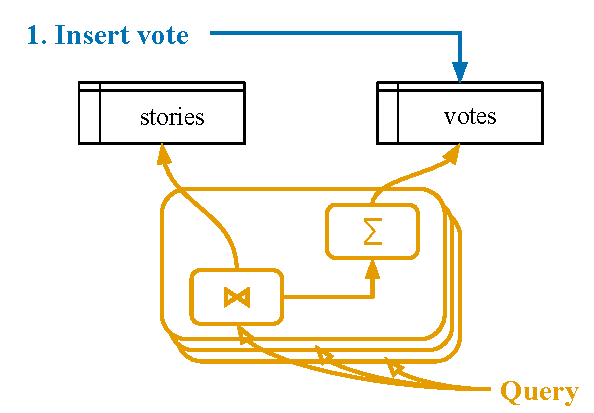
\includegraphics{diagrams/Motivation Classic DB.pdf}
  \caption{Application query execution against a traditional database. Each
  application query runs in isolation, and may perform the same work
  (\textbf{\color{set2}orange}) repeatedly. Writes do little work
  (\textbf{\color{set1}blue}), even though they are less frequent in many
  applications.}
  \label{f:motivation-classic}
\end{figure}

Figure~\vref{f:motivation-classic} shows how application queries function at a
high level in the traditional model: each query the application issues executes
the query plan, represented by an aggregation and a join in the figure. Multiple
concurrent queries execute independently, even if they run the same query.

\section{Existing Solutions}
\label{s:existing}

\begin{figure}
  \centering
  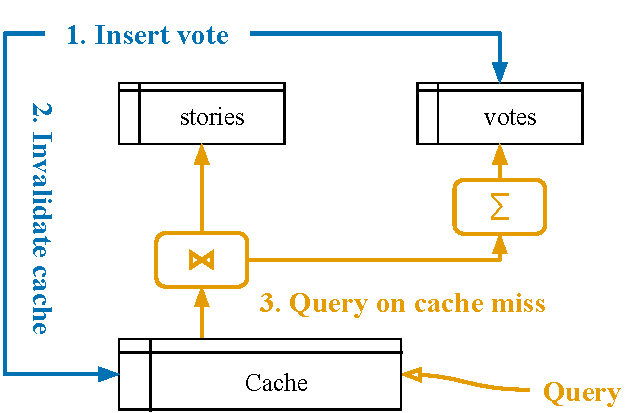
\includegraphics{diagrams/Motivation Ad Hoc Cache.pdf}
  \caption{Application query execution against a cache in front of a database.
  Application queries first check for cached results, and only execute database
  queries if the results are not cached. The application invalidates cached
  results so that later reads see the effects of new writes. The application
  logic for both reads (\textbf{\color{set2}orange}) and writes
  (\textbf{\color{set1}blue}) is more complex.}
  \label{f:motivation-adhoc}
\end{figure}

To mitigate the lackluster performance of databases for these workloads,
application authors often resort to ad hoc, error-prone
techniques~\cite{ad-hoc-caching} to exploit their applications' workload
patterns. They change their database schemas by placing and updating computed
values in the database tables, or introduce key-value stores that \textit{cache}
the result of expensive queries as shown in Figure~\vref{f:motivation-adhoc}.
All these techniques introduce significant application complexity: the
application authors must include logic to ensure that the auxiliary derived
state remains up to date as the underlying data changes, that clients do not all
flood the database when results are not available in the cache, and that
concurrent access to the database and the cache never leaves the system in an
inconsistent state.

Existing systems from industry~\cite{facebook-memcache, tao, flannel} and
academia~\cite{txcache, cachegenie, casql-consistency-thesis, pequod} have
chipped away at this problem, but are often lacking in important ways. Some
require significant developer effort, and are infeasible to implement for any
but the largest companies. Some support only a restricted set of queries, or
only provide infrastructure for developers to implement caching themselves. Many
keep the cache up to date only by evicting old results, and cannot update
existing results in-place, which is wasteful.

% Noria replaces caching \emph{logic}, not caching just caching \emph{systems}.

Eons ago~\cite{relational-materialized-views,stonebraker-views}, the database
community introduced \textit{materialized views} as an answer to the problem of
how to execute queries that are too slow to execute on demand. Materialized
views store the contents of \textit{views} (i.e., named queries) which makes
those queries faster to execute~\cite{materialized-views}. The materialized
views can then be \textit{maintained} incrementally, meaning results are updated
in-place, rather than invalidating stored results or re-executing queries from
scratch when the underlying data changes~\cite{materialized-survey}.

\begin{figure}[h]
  \centering
  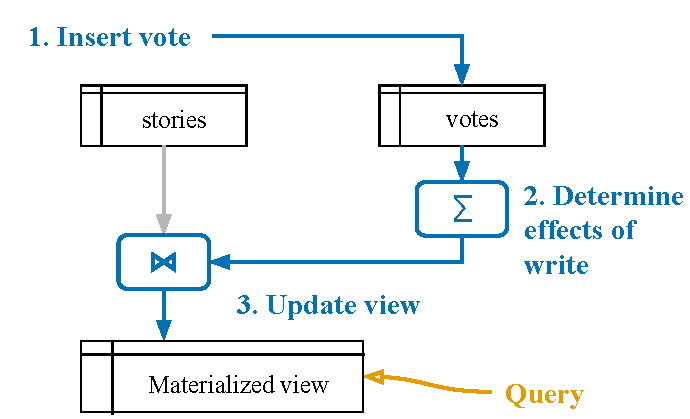
\includegraphics{diagrams/Motivation Materialized Views.pdf}
  \caption{Application query execution against a materialized view. Application
  queries only hit the view, which gives simple yet fast reads
  (\textbf{\color{set2}orange}). The database must determine the effects of
  every write and update the views to reflect changes
  (\textbf{\color{set1}blue}).}
  \label{f:motivation-materialized}
\end{figure}

Figure~\vref{f:motivation-materialized} shows an approximate architecture for an
incrementally-maintained materialized view system. The system updates the
materialized results in response to application writes, and reads access only
the stored results. Sadly, few commercially available databases support
materialized views, and the ones that do have significant
restrictions~\cite{mssql-materialized-view-restrictions}.

State-of-the-art research systems support flexible materialized
views~\cite{dbtoaster,materialize}, but do not support low-latency reads. In
these systems, reads cannot access the materialized view directly, and must
synchronize with the write-processing pipeline to get query results. Many of
these systems are also restricted to a predeclared set of queries, and cannot
incorporate changes to application queries without restarting.

Most materialized view systems do not have the ability to evict infrequently
accessed state that accumulates over time. They thus function poorly as a
replacement for a cache: infrequently accessed results cannot be evicted, and
reads must wait on writes. Dynamic materialized
views~\cite{dynamic-materialized-views, partially-materialized-views} allow the
application to materialize only a subset of each view. This enables limited
eviction, but is cumbersome for the application to manage, and only allows
coarse-grained eviction decisions (\S\ref{s:disc:emulating}).

\section{Approach: Partial State}
\label{s:approach}

Materialized views represent an ``almost there'' solution to automatic caching.
They provide a great foundational mechanism for storing and maintaining query
results efficiently in a way that meshes well with how applications already
work: by issuing SQL queries. What is missing to make materialized views a
viable replacement for the ad hoc caching strategies today's applications employ
is a way to make the materialized views more dynamic. Specifically, to serve as
a good cache-substitute, materialized views must support efficiently adding new
queries and evicting old results at runtime.

To bridge the gap, this thesis proposes \textit{partially materialized
state}\footnote{The database literature sometimes refers to a view where only
some columns are materialized as ``partially
materialized''~\cite{partially-materialized}. This meaning of the term is
unrelated to the use of the term in this thesis.}, or partial state for short.
Partial state lets entries in materialized views be marked as \textit{missing},
and introduces \textit{upqueries} to compute such missing state on-demand.
This allows new queries to be added efficiently by leaving the initial
materialized view empty, and populating the view only in response to application
queries. Furthermore, as the application loses interest in old query results,
those results can be evicted to reclaim memory, which can in turn be used to
cache more important query results. In essence, partial state enables
materialized views to function like caches.

In the proposed work, the system model still looks like
Figure~\vref{f:motivation-materialized}, except that the materialized view also
contains parameters whose value the application supplies at runtime. Queries to
the materialized view can then \emph{miss} for a given parameter value, just
like in a cache. When they do, the database internally fills in the missing
state before it responds to the application. If the application later executes
the same query, the cache holds the result. Over time, the database evicts
infrequently accessed results to save memory and to avoid the overhead of
maintaining results the application is no longer interested in.

\section{Partial State in Noria}
\label{s:intro:noria}

The thesis includes an implementation of partial state in Noria, a
state-of-the-art materialized view system that is already optimized for
read-heavy, dynamic web applications~\cite{noria}. Noria uses \textit{dataflow}
internally to maintain its materialized views, a system architecture that allows
fast and distributed computation over a stream of data changes. Dataflow
represents computational dependencies as a directed acyclic graph where edges
represent data dependencies, and vertices represent computations (like
aggregations or joins) over the data that arrives over the incoming edges.
Partial state upqueries flow ``up'' this dataflow, in the opposite direction of
the data, and trigger the retransmission of past state in the case of a cache
miss. The resulting retransmissions then use the existing Noria dataflow to
process the responses and fill in missing state. This avoids the need for
separate logic for serving cache misses and maintaining already cached state,
and simplifies the implementation.

\section{Contributions}
\label{s:contrib}

The main contributions of this thesis are:

\begin{itemize}
 \item A model for, and implementation of, partial state in a dataflow-based
   materialized view system.
 \item Upqueries\,---\,a mechanism that populates missing state on demand.
 \item An analysis of the inconsistencies that arise when introducing partial
   state to a distributed, high-performance stateful dataflow processing system
    where updates can race with one another, and with upqueries.
 \item Techniques for overcoming those inconsistencies while preserving system
   correctness, performance, and scalability.
 \item Micro and macro evaluations of the performance and memory benefits of
   partial state. Experimental results suggest that the presented system
    increases supported application load by up to $20\times$ over MySQL, and
    reduces memory use by up to $\sfrac{2}{3}$ compared to existing approaches.
\end{itemize}

\section{Reading Guide}
\label{s:read}

The rest of the dissertation is organized as follows: Chapter~\ref{s:noria}
describes the Noria dataflow system. Chapter~\ref{s:partial} introduces the
partially stateful dataflow model. Chapter~\ref{s:correct} describes additional
mechanisms that are needed to ensure that partially stateful dataflow produces
correct query results. Chapter~\ref{s:impl} details some of the implementation
decisions in the thesis prototype. Chapter~\ref{s:eval} evaluates Noria's
implementation of partial state on a realistic application query workload.
Chapter~\ref{s:related} explores related work. Chapter~\ref{s:disc} discusses
shortcomings of, and alternatives to, partial state. Finally,
Chapter~\ref{s:future} outlines future work on partial state.

For readers that are unfamiliar with database queries, materialized views,
dataflow, and application caching, but would still like to understand roughly
what this thesis is about, Appendix~\ref{s:simple} starting on
page~\pageref{s:simple} is for you.


\chapter{Background: Noria}
\label{s:noria}

In this thesis, partial state is implemented in Noria~\cite{noria}, a stateful,
dynamic, parallel, and distributed dataflow system designed for the storage,
query processing, and caching needs of typical web applications. Because of the
strong connection between Noria and partial state, this chapter describes the
design and implementation of Noria in sufficient depth to understand the
remainder of the thesis.

\section{High-Level Overview}

Noria runs on one or more multicore servers that communicate with clients and
with one another using RPCs. A Noria deployment stores both \emph{base tables}
and \emph{derived views}. Roughly, base tables contain the data typically stored
persistently in relation tables, and derived views hold data an application
might choose to cache to improve performance.

Compared to conventional database use, Noria base tables might be smaller, as
Noria derives data that an application may otherwise pre-compute and store
denormalized in base tables for performance. Noria stores base tables
persistently on disk, either on one server or sharded across multiple servers.
Views, by contrast, are likely larger than a typical cache footprint, because
Noria derives more data, including some intermediate results. Noria stores views
in memory.

Noria's interface resembles parameterized SQL queries. The application supplies
a \emph{Noria program}, which registers base tables and views with parameters
supplied by the application when it retrieves data. The Noria program includes
base table definitions, \emph{internal} views used as shorthands in other
expressions, and \emph{external} views that the application later queries
(the next section gives an example). It can be thought of as an extended schema
for the application that includes its queries.

Noria differs substantially from traditional databases in how it executes
queries. Rather than compute a query's results on demand when the application
executes it, Noria does so when the query view is defined. Noria then caches, or
\emph{materializes}, the contents of that view, and serves queries to that view
directly from that cache. To keep the materialized view current, Noria
internally instantiates a dataflow program to continuously process the
application's writes and update the views as appropriate.

This kind of view materialization makes Noria particularly well-suited for
read-heavy applications that tolerate eventual consistency, since it shifts
query execution cost from reads, which are frequent, to writes, which are
infrequent.

\paragraph{Materialization.}
Throughout this thesis, the word materialization is often used as a noun. In the
context of Noria, a materialization refers to any derived computation result
that Noria explicitly stores, not just materialized views. Or, more precisely,
Noria may choose to materialize intermediate results, such as the current value
of an aggregation, which do not represent any of the application's queries.
These intermediate materializations are still views\,---\,they have a schema and
consist of rows\,---\,but do not reflect any named views that the application
has created.

\section{Application Interface}

\begin{listing}[h]
  \begin{minted}{sql}
/* base tables */
CREATE TABLE stories (id int, title text);
CREATE TABLE votes (story_id int, user int);
/* internal view: vote count per story  */
CREATE INTERNAL VIEW VoteCount AS
  SELECT story_id, COUNT(*) AS vcount
    FROM votes GROUP BY story_id;
/* external view: story details */
CREATE VIEW StoriesWithVC AS
  SELECT id, author, title, url, vcount
    FROM stories
    JOIN VoteCount ON VoteCount.story_id = stories.id
   WHERE stories.id = ?;
  \end{minted}
  \caption{Noria program for a key subset of the Lobsters news
           aggregator~\cite{lobsters} that counts users' votes for stories.}
  \label{l:vote-src}
\end{listing}

Listing~\vref{l:vote-src} shows an example Noria program for a news aggregator
application where users can vote for stories.

To retrieve data, the application supplies Noria with an external view
identifier (e.g., \texttt{StoriesWithVC}) and one or more sets of parameter
values (\texttt{?} is a parameter). Noria then responds with the records in the view that match those
values. To modify records in base tables, the application performs insertions,
updates, and deletions, similar to a SQL database. Data is represented as
structured records in tabular form~\cite{spanner, bigtable}.

The application may change its Noria program to add new views, to modify or
remove existing views, and to adapt base table schemas. When it does, Noria
adapts the running dataflow to incorporate the changes without restarting the
dataflow engine.

Unlike the iterative or graph computations that are the focus of other dataflow
systems~\cite{naiad, differential-dataflow}, Noria focuses entirely on
relational operators. Noria supports much, but not all, SQL.

\section{Dataflow Execution}

To keep its materialized views from growing stale as the underlying data
changes, Noria uses dataflow. Noria compiles all the application queries into a
joint dataflow program, which it routes all application writes through. The
dataflow is a directed acyclic graph of relational operators such as
aggregations, joins, and filters. Base tables are the roots of this graph, and
external views form the leaves. Noria extends the graph with new base tables,
operators, and views as the application adds new queries.

When an application write arrives, Noria applies it to a durable base table and
injects it into the dataflow as an \emph{update}. Operators process the update
and emit derived updates to their children; eventually updates reach and modify
the external views. Updates are \emph{deltas}~\cite{roll, differential-dataflow}
that can add to, modify, and remove from downstream state. Deltas are similar to
mathematical multisets, or ``bags'', except that the multiplicity of an element
may be negative. For example, a count operator emits deltas that indicate how
the count for a key has changed; a join may emit an update that installs new
rows in downstream state; and a deletion from a base table generates a
``negative'' update that revokes derived records. Negative updates remove
entries when Noria applies them to state, and retain their negative ``sign''
when combined with other records (e.g., through joins). Negative updates hold
exactly the same values as the positives they revoke and follow the same
dataflow paths.

The combined deltas emitted by an operator from the beginning of time
constitutes the operator's current state. This state may not be stored anywhere,
or the delta stream may be \textit{materialized}, in which case the current
multiset of records is stored by the system. It is helpful to think of
\emph{edges} as being materialized, rather than operators or views, since a
materialization is exactly equivalent to the evaluation of the deltas that have
flowed across that edge.

Noria supports \emph{stateless} and \emph{stateful} operators. Stateless
operators, such as filters and projections, need no state to process updates;
stateful operators, such as count, min/max, and top-$k$, maintain state to avoid
inefficient re-computation of aggregate values from scratch. Stateful operators
also keep one or more indexes to speed up operation. Noria adds indexes based on
\emph{indexing obligations} imposed by operator semantics; for example, an
operator that aggregates votes by user ID requires a user ID index to process
new votes efficiently. Noria's joins are stateless, but require that the state
of their inputs be materialized to allow an update arriving at one input to join
with all relevant state from the other.

\subsection*{Example Execution}

\begin{figure}[t]
  \centering
  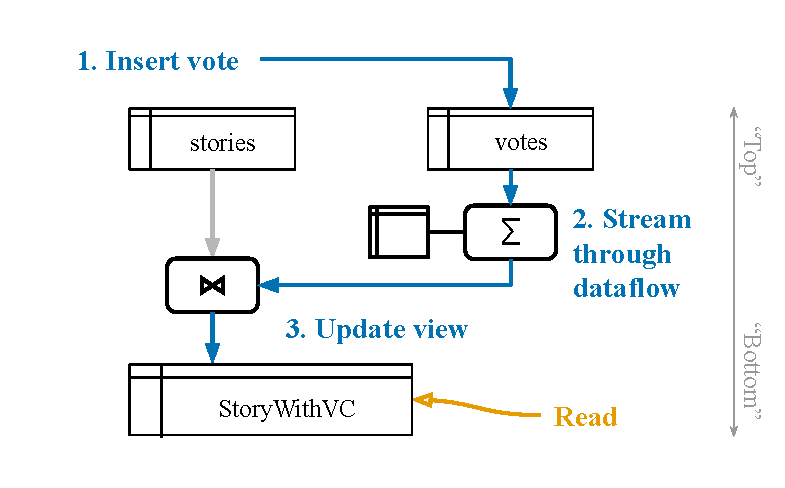
\includegraphics{diagrams/Example Execution.pdf}
  \caption{Noria's dataflow program to maintain Listing~\ref{l:vote-src}. Text
  describes the update path highlighted in \textbf{\color{set1}blue}. The
  dataflow inputs are considered the ``top'' of the dataflow, and the leaves are
  at the ``bottom''. Parents are ``upstream'' of their ``downstream'' children.}
  \label{f:example-exec}
\end{figure}

Figure~\vref{f:example-exec} shows the dataflow that Noria constructs for
maintaining the Noria program in Listing~\vref{l:vote-src}. At the top are the
entry points into the dataflow\,---\,the operators that represent the schema
base tables\,---\,one for the \texttt{stories} table, and one for the
\texttt{votes} table. Connected to the \texttt{votes} table is a counting
aggregation operator ($\sum$), which corresponds to the internal
\texttt{VoteCount} view. It feeds into a join operator ($\bowtie$), which in
turn connects to the external \texttt{StoryWithVC} view.

To understand how Noria uses this program to maintain the external view,
consider what happens when the application adds a new vote. The application
performs the insertion by introducing the write into the dataflow as a
single-row update with a positive sign at the \texttt{votes} operator. Noria
stores the update to durable storage, and then forwards the update as-is to its
children; in this case, the count operator.

The count operator performs a lookup into its own output state for the current
count of the new row's group by column value. The semantics of a count is that
an insertion increments that number by one, so the operator emits a replacement
update for the old state. In particular, the update it produces contains a
negatively-signed delta with the old count, and a positively-signed delta with
the updated count. Both deltas include the group by column value.

The replacement is represented as a separate negative and positive delta since
the two may take different paths through the dataflow. For example, a downstream
filter might filter out stories with a vote count below a given threshold. If
the latest vote makes the count exceed the threshold, the negative delta should
not flow down the dataflow past the filter, since there is nothing there for it
to revoke. However, the positive delta should, since the story (with its updated
count) now passes the filter.

When the join operator receives this replacement update from the count, it
performs a lookup into its other ancestor, \texttt{stories}, for records that
match the join column value of each delta of the incoming update. In this case,
both deltas (the negative one and the positive one) have the same story
identifier as the join value, and the lookup finds only a single
record\,---\,the matching story. The operator then joins each delta with each
matching result. This produces an update that (still) contains one negative and
one positive delta, but where each delta now includes additional columns from
the \texttt{stories} table.

Ultimately, this two-delta update arrives at the operator that represents the
external \texttt{StoryWithVC} view. The changes from the update are applied one
by one, with the negative delta removing the entry in the view with the old vote
count, and the positive delta adding the replacement entry.

\section{Consistency Semantics}
\label{s:noria:consistency}

To achieve high parallel processing performance, Noria's dataflow avoids
global progress tracking or coordination. An update injected at a base table
takes time to propagate through the dataflow, and the update may appear in
different views at different times. Noria operators and the contents of its
external views are thus \emph{eventually-consistent}. Eventual consistency is
attractive for performance and scalability, and is sufficient for many web
applications~\cite{eventually-consistent, facebook-memcache, pnuts}. In
particular, Noria ensures that if writes quiesce, all external views eventually
hold results that are the same as if the queries had been executed directly
against the base table data.

Ensuring even this relatively weak property requires some care. Like most
dataflow systems, Noria requires that operators are deterministic functions over
their own state and the inputs from their ancestors. Furthermore, operators must
be distributive over delta addition\footnote{$d_1 + d_2$ produces the union of
all rows in $d_1$ or $d_2$ with the signed multiplicity of each row equal to the
algebraic sum of that row's signed multiplicity in $d_1$ and $d_2$.} so that
evaluating the query using tuple-at-a-time processing is equivalent to
evaluating the whole query at once. Finally, Noria operators must be commutative
so that operators with multiple inputs, like unions and joins, can process their
inputs in any order without coordination\footnote{Maintaining eventual
consistency with partial state requires additional mechanisms, as discussed in
\S\ref{s:correct}.}. The standard relational operators that Noria supports all
have this property.

\paragraph{How Eventual?}
While Noria does not guarantee exactly when a write is visible in a given view,
the time between when a write is acknowledged and when it becomes visible should
be short. A view is stale only while the write propagates through the dataflow,
so the time before the write manifests depends only on the height and complexity
of the dataflow for the view in question.

\subsection{Prefix Consistency}

Eventual consistency is a woefully vague consistency model\,---\,an eventually
consistent system is allowed to do anything, or nothing at all, as long as reads
\emph{eventually} all return the same value. Most definitions of eventual
consistency also require that that same value reflects the writes issued to the
system, but not all. In practice, eventual consistency is often ``good enough''
despite giving few \emph{guarantees}, and many eventually consistent systems
appear strongly consistent most of the time~\cite{eventual}.

Noria upholds three additional safety properties:

\begin{invariant}
  \label{i:no-spurious}
  All reads reflect each upstream base table change at most once.
\end{invariant}

\begin{invariant}
  \label{i:prefix-consistency}
  A read that observes all effects of a given base table change also observes
  all earlier changes to that same base table.
\end{invariant}

\begin{invariant}
  \label{i:no-backsies}
  A read issued at time $t$ and again at time $t' > t$ observes the effects of
  at least as many updates at $t'$ as at $t$.
\end{invariant}

Invariant~\ref{i:no-spurious} ensures that views include no duplicate or
spurious results. Essentially, it guarantees that view results represent data
that is in the base tables, and no other data.

Invariant~\ref{i:prefix-consistency} ensures that when the system makes
progress, it does so in a sane manner. If the application issues two writes
$w_1$ and $w_2$ to a base table in that order, then it will not see $w_2$
reflected but not $w_1$.

Invariant~\ref{i:no-backsies} ensures that \emph{if} the system makes progress,
that progress persists\,---\,Noria cannot expose the effects of an update, and
then roll back those effects at a later time. Of course, if a later update
happens to mask the effects of the earlier update, that is fine\,---\,the
invariant is still preserved.

Informally, these three invariants taken together establish a sort of per-table
\emph{prefix consistency}. For each base table $b$ that connects to a given view
$v$, there exists some time $t$ such that all changes in $b$ that precede $t$
manifest exactly once when reading from $v$. Effects from changes that succeed
$t$ may manifest fully, partially, or not at all. As Noria continues executing
its dataflow, $t$ increases, and more changes manifest fully.

Note that prefix consistency applies \emph{per base table}. If the application
writes $w_1$ to \texttt{votes} and then $w_2$ to \texttt{stories}, the effects
of $w_2$ may manifest downstream before $w_1$ does.

\subsubsection*{Sharding and Consistency}

When Noria's sharding feature is enabled, base tables are also sharded, which
complicates the meaning of \emph{earlier} from
Invariant~\ref{i:prefix-consistency}. In particular, concurrent updates to
different shards of the same base table do not happen before or after each other
in any well-defined way. Thus, a read that observes the effects of one base
table change may not observe the effects of another change that happened before
if that other update was issued to a different shard of the base table.

Noria's views can also be sharded, in which case the shards are updated
independently. If the effects of an update are present in one shard of a view,
they may not yet have manifested in another shard of that same view.

\subsection{What Can Go Wrong?}

Noria's eventual consistency can lead to reads producing strange results
under certain circumstances in stream processing
systems~\cite{materialize-eventual}. As an example, consider the query in
Listing~\vref{l:always-wrong}. If the maximum value changes frequently enough,
then the outer and inner query may be perpetually ``out-of-sync''. The current
maximum may not yet be present in the outer query, or a new maximum value may
not yet be present in the inner query. The net result is that the result set of
the query would be empty, even though a traditional database would never yield
an empty query result.

\begin{listing}[h]
  \begin{minted}{sql}
    SELECT data.key FROM data
    WHERE data.value IN
      (SELECT MAX(data.value) FROM data)
  \end{minted}
  \caption{Query that may perpetually produce no results in Noria.}
  \label{l:always-wrong}
\end{listing}

If the max value changes less frequently, and Noria has time to process a new
update through both dataflow paths (the inner and the outer) before the maximum
changes again, Noria will produce the expected non-empty query result. But
nonetheless, the application author probably did not expect that this query
could return an empty result set, however briefly.

Exactly how strange these phenomena become, and how frequently they manifest,
depends on the nature of the queries and the updates. For example, queries that
access each base table only once will produce results that are stale, but never
results that do not match the results a traditional database would have given
given the same base table data. Queries with self-joins on the other hand are
particularly prone to these temporary inconsistencies. For example, a join that
computes a parent-child relationship between records may briefly reflect a new
record as a child, but not as a parent, or vice-versa.

These inconsistencies arise due to race conditions in the dataflow graph. In
particular, if two deltas resulting from a single upstream change race against
each another down different dataflow paths that later converge, one delta will
be applied to the final view before the other. This leaves the view in an
intermediate state where a partial effect of the original update can be observed
until the other delta arrives.

\begin{listing}[h]
  \begin{minted}{sql}
    SELECT id, state FROM data WHERE state = 1
    UNION
    SELECT id, state FROM data WHERE state = 2
  \end{minted}
  \caption{Query that may produce duplicates briefly in Noria.}
  \label{l:duplicates}
\end{listing}

Listing~\vref{l:duplicates} gives an example of a query with this kind of race
condition. Imagine that the application changes the \texttt{state} where
\texttt{id = 42} from 1 to 2. In Noria, this is represented by a removal of the
now-outdated record, and an addition of the updated record. The removal follows
the dataflow path for \texttt{WHERE state = 1}, while the addition follows the
dataflow path for \texttt{WHERE state = 2}. One of those updates will arrive
first at the union, and the materialized view. If it is the removal, then reads
will not see a record with \texttt{id = 42} until the addition is processed.
Conversely, if the addition arrives first, reads will see two records with
\texttt{id = 42} (one with \texttt{state = 1} and one with \texttt{state = 2})
until the removal is processed.

To mitigate these kinds of inconsistencies, Noria would either need to enforce
that no reads can happen between the application of one ``half'' and the other,
or somehow hide the partial effects of applying only the first part. The former
requires reads to flow through the dataflow, or at least synchronize closely
with it, which would likely come at a penalty to read latency. The latter would
be provided through something akin to multi-version concurrency control, which
allows low-latency reads, but adds significant system complexity.

Instead, Noria works under the assumption that queries that produce these
inconsistencies are rare for Noria's target applications, or that application
developers direct those queries where strong consistency is necessary to other,
better suited systems.

\section{Parallelism}

Servers have many cores, and any high-performance system must be able to take
advantage of these cores to take full advantage of the hardware. Noria does so
in several ways. First, it allows reads to happen independently from any number
of threads concurrently. Second, it allows different threads to process writes
in disjoint parts of the dataflow concurrently. And third, it supports sharding
individual operators, or cliques of operators, so that multiple threads can
process disjoint subsets of the data concurrently through the same dataflow
segment. These three mechanisms are described further below.

\subsection{Read Independence}

Since Noria is designed for read-heavy workloads, its architecture is optimized
to allow reads to go ahead at full speed whenever possible. In particular, Noria
does not synchronize reads with reads \emph{or} writes\footnote{If a read
encounters missing partial state, as described in the next chapter, some
lightweight synchronization is needed to communicate the missed key}.

This is achieved through a concurrency primitive that maintains two instances of
each materialized view, with deduplication between them. Reads go to one view,
and writes to the other. Readers see updates to the view only when a writer
exposes those changes explicitly\,---\,the writer flips an atomic pointer to the
other view, and then waits for all readers to exit the old view before modifying
it again. This flip can be done on every update, as Noria currently does, or
only occasionally to amortize the cross-core communication penalty and the wait
period for the writer. Crucially, readers do not take locks, and generally
operate only on core-local cache lines.

This design allows Noria to use any number of threads to serve reads from any
view. As long as there are cores available, Noria can use additional threads to
perform view lookups, as well as low-level networking work like request
serialization and read/write system calls.

\begin{inprogress}
  Should I include an Appendix that explains how evmap works in further detail?
\end{inprogress}

\subsection{Partitioning}

The dataflow model is attractive because it is inherently streaming, and thus
particularly well-suited for distributed deployments. Operators are independent
and communicate only through their streams, so Noria can easily place them
on different cores, or hosts, and use the appropriate messaging fabric to
connect them.

Tot take advantage of this, Noria divides the dataflow graph into a number of
sub-graphs called \textit{thread domains}. Only a single thread can process
updates in a given thread domain at a time (except with sharding; see below),
and any update that enters a thread domain is processed to completion within
the domain before another update is processed.

Noria never shares state between thread domains, which means that state access
is not guarded by locks. Thread domains communicate with one another only
through messages across the edges of the dataflow, or in the case of upqueries,
by sending messages through dedicated upquery paths set up by the partial
subsystem. All such communication can happen either over the network if the
other thread domain is on a different host, or over an in-memory channel if it
is local.

Since thread domains share nothing, Noria duplicates state across boundaries
when needed. For example, a join operator at an incoming edge of a thread domain
must be able to perform lookups into the state of its ancestor, which sits in a
different thread domain. In such a case, Noria will create a thread-local copy
of the join's ancestor's state that it can use locally. Noria's thread domain
assignment heuristics will attempt to draw domain boundaries  such that this
kind of duplication is unnecessary. For example, it will prefer drawing a domain
boundary just before an aggregation (which does not need to look up in the state
of its ancestor), and avoid drawing a domain boundary just before a join.

\subsubsection{Join Consistency}
\label{s:join-state-dupe}

The thread-local copy of lookup state, such as for joins, serves a second
purpose: it mitigates a race condition that would otherwise arise from
cross-domain state lookups. Consider a join operator J with parents L and R. If
R's state was in a different domain than J, then the following can happen:

\begin{enumerate}
  \item R receives and incorporates a delta $d_R$ that adds row $r_R$.
  \item J receives a delta $d_L$ from L that adds row $r_L$.
  \item J performs a lookup into R's state based on $d_L$'s join key. The result
        includes $r_R$, so J emits a delta that adds $r_L \bowtie r_R$.
  \item $d_R$ arrives at J.
  \item J performs a lookup into L's state based on $d_R$'s join key. The result
        necessary includes $r_L$, so J emits a delta that adds $r_L \bowtie r_R$
        a second time.
\end{enumerate}

This issue arises because the lookups bypass deltas that are in-flight between R
and J. The lookups thus get to observe ``the future''. This erroneously causes J
to incorporate the same data at two points in time, which violates
Invariant~\ref{i:no-spurious}.

Multi-version concurrency control could likely be used to solve this problem,
but would be heavyweight solution that also requires much more significant
synchronization. Especially if J and R happen to be on different physical hosts.
Duplicating R's state across the domain boundary avoids the problem\,---\,since
thread domains process all updates within the domain to completion, there can be
no deltas in flight between R and J, and the lookup will never observe future
state.

\subsection{Sharding}
\label{s:noria:sharding}

To accommodate applications with such a high volume of writes that the
processing at a single operator is a bottleneck, Noria supports sharding an
operator. Multiple threads split the work of handling updates to a sharded
operator, and operate like independent, disjoint parts of the dataflow.

Noria implements static hash partitioning: it decides how to shard an operator
when the operator is added to the dataflow, and this sharding does not change
over the runtime of the application. Sharding by value ranges and adjusting the
sharding dynamically is left for future work.

Noria shards operators primarily based on how they access state. For example, an
aggregation that performs lookups into its own state is sharded by the key
column of those lookups. Any other sharding would mean that processing one
update would require coordination among all shards. A join is sharded by the
join key for the same reason. Base tables are sharded by the table's primary
key. Operators that do not perform lookups (e.g., unions) continue the sharding
of their ancestors to avoid unnecessary resharding.

To shard an operator, Noria introduces two additional nodes in the dataflow: a
\emph{sharder} placed upstream of the sharded operator, and a \emph{shard
merger} downstream of it. The sharder routes incoming updates to the appropriate
shard of the sharded operator, and the shard merger is a union operator that
combines the output of all the shards to a single downstream output stream.
Noria then eliminates unnecessary sharders and shard mergers, such as if an
operator and its ancestor are sharded the same way.

Sharding boundaries are also natural thread boundaries, though two connected
thread domains may also be sharded differently. Or, phrased differently, Noria
may partition a chain of operators that are all sharded by the same column into
multiple thread domains to increase parallelism.

\begin{comment}
  Sharding is tracked based on "ultimately source column". (column tracing)
\end{comment}


\chapter{Partial State}
\label{s:partial}

Noria without partial state, as described in \S\ref{s:noria}, uses significant
amounts of memory. All results for all queries must be materialized, and unlike
traditional caching approaches, unimportant cached results are not evicted to
free up memory. To address the high memory use of traditional materialized
views, this thesis proposes \textit{partially materialized state}, often
shortened to partial state. Partial state enables Noria to store and maintain
only a subset of a materialized view's contents, and to compute missing state on
demand. Partial state also enables Noria to implement eviction, so that the
materialization cost is kept low even as the underlying workload changes.

This chapter discusses the partially stateful model and its components. The next
chapter examines the practical challenges that arise when partial state is
implemented in a dataflow system.

\section{Missing State}
\label{s:missing}

Partial state allows state to be \textit{missing}. Missing state indicates that
a particular value is not yet known, and must be computed on demand if the
application queries for it. State can be marked as missing both in state that is
internal to the dataflow, like the state of an aggregation, and in externally
visible state like Noria's query result caches.

With partial state, most Noria state starts out as missing, and is populated
according to what data the application queries for. This also allows Noria to
quickly adopt new views, since in the common case no computation need happen
when additional operators are added.

\begin{figure}
  \centering
  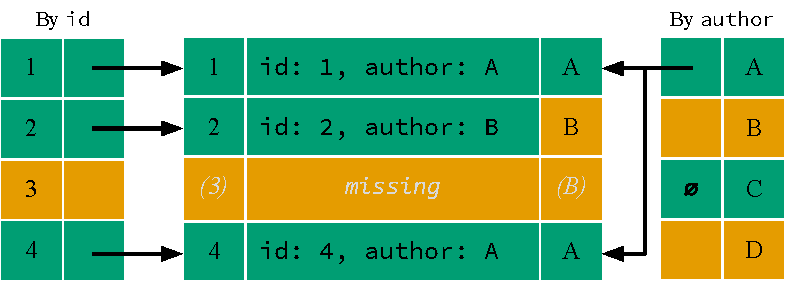
\includegraphics{diagrams/Indexing.pdf}
  \caption{Multiple indexes in a single view in Noria. Even though \emph{some}
  rows for author B are \textbf{\color{set3}present}, some are
  \textbf{\color{set2}missing}, so the entry for B is missing in the
  \texttt{author} index. Even though there are no rows for author C, the index
  entry is not marked as missing, which would happen if Noria has already
  checked that there are indeed no rows in the base tables that match author C.}
  \label{f:indexing}
\end{figure}

Missing state manifests as missing entries in indices. Indexes over a given
state are either all partial or none of them are. This may seem strange given
how indices work in traditional relation databases. Figure~\vref{f:indexing}
gives an example of two partial indices over a view that holds a unique story
identifier and the story's author. One index is over the primary key column
\texttt{id}, and one is over the story author. Even though some rows with author
B are present, the index entry for author B is still considered missing, as not
\emph{all} rows with author B are present. This is necessary, as otherwise a
query for stories authored by B would return a result with missing rows.

While there are no rows for authors C or D, C is considered complete because
Noria has checked upstream that there are indeed no stories written by C. For D,
Noria has not yet done an upstream check, and therefore does not know what the
true result set is.

If Noria encounters missing state while processing an update, the update must
not affect query results that the application has indicated interest in. In such
a case, Noria has two options: eagerly compute the missing state before
proceeding, or discard the update. To avoid unnecessarily maintaining
unimportant cached results, Noria drops updates in this case.

An important corollary of the above is that partial state must be enabled
on all stored state \emph{below} any partial state. It is illegal for the
dataflow to contain state for two nodes $A$ and $B$ where $A$ is an ancestor of
$B$, $A$ uses partial state, and $B$ does not use partial state. To see why,
consider what would happen if an update arrives at $A$ for a missing entry. $A$
would discard that update, and $B$'s state would never reflect it and grow
perpetually stale.

\section{Upqueries}
\label{s:upqueries}

If an application requests data that is found to be missing, Noria issues an
\textit{upquery} to compute the requested data. Upqueries flow ``up'' the
dataflow graph, towards the base tables at the ``top'', and constitute a request
for the target of the upquery to replay past data. Upqueries may recurse if the
requested state is not available at the initial target.

The response to an upquery takes the form of a regular dataflow update that
flows down the dataflow. It combines all past deltas pertinent to the upquery
into a single update, and holds only positive deltas that represent the current
set of relevant records.

Operators are not generally aware if they are processing an update that resulted
from an upquery response. The upquery response flows in-line with other dataflow
updates, and follows the edges of the dataflow. However, upquery responses are
special in two key ways. First, they only propagate along edges towards the
operator that issued the upquery, so that one upquery does not populate the
relevant data in the state of \emph{every} operator. And second, if an operator
encounters missing state while processing an upquery response update, it does
\emph{not} discard that update as it would a regular dataflow update. Instead,
it eagerly does the work necessary to fill the missing state and then process
that update.

When an application query encounters missing state in a view, Noria needs to
know what upqueries to issue to fill that state. The set of upqueries for each
view is that view's \textit{upquery plan}. Noria determines upquery plans by
analyzing each view's query when the application first installs that view, and
deciding how best to recompute its results. It does so by finding all
\emph{possible} upquery plans, choosing among them, and then informing all
involved domains of the chosen plan. There may be multiple possible candidates
if there are multiple equivalent ways to compute the missing state, such as by
changing the direction in which joins are executed as explained below.

\subsection{Key Provenance Tracing}

To determine what upqueries can reconstitute missing entries in a given index,
Noria must trace the view's parameter column (the \texttt{?} in the query) back
to a column in upstream state. The intuition here is that in order to answer the
application's query of ``give me the results where column $C$ has value $x$'',
Noria must be able to replay rows where $C = x$ from somewhere. Or, phrased
differently, when the output for $C = x$ is missing, Noria must have a way to
get the inputs that \emph{generate} $C = x$. As an example, if a view counts
books by a given author, and the current count for author $a$ is missing, Noria
must be able to somehow produce all books by author $a$.

\begin{figure}[t]
  \centering
  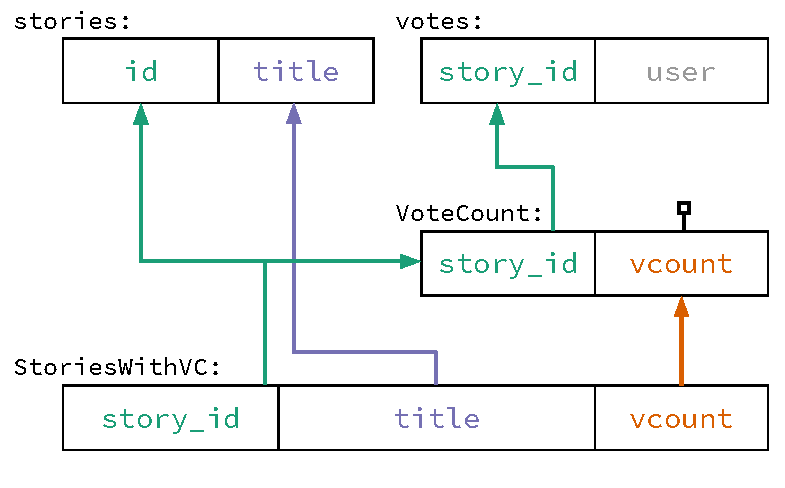
\includegraphics{diagrams/Key Provenance.pdf}
  \caption{Key provenance for each column in the \texttt{StoriesWithVC} view
  from Listing~\ref{l:vote-src}. Notice that \texttt{\color{set3}story\_id} has
  multiple base table origins, and \texttt{\color{set2}vcount} does not trace
  back to any base table columns. The query only uses
  \texttt{\color{set3}story\_id} as a parameter, so only its provenance is used
  to choose the upquery path.}
  \label{f:key-prov}
\end{figure}

More generally, in order to recompute the results where $C = x$ in some view
$V$, Noria must determine the \textit{key provenance} of $C$; where $C$ ``came
from''. Noria computes key provenance by tracing columns ``up'' the dataflow to
where they originate, which results in a \textit{provenance graph}.
Figure~\ref{f:key-prov} shows the provenance graph for the
\texttt{StoriesWithVC} view from Listing~\vref{l:vote-src}, and illustrates two
important properties of key tracing:

\begin{enumerate}
  \item An output column may trace to multiple input columns if it corresponds
    to the join column in a join, or if it passes through a union. The
    provenance of the \texttt{story\_id} column, for example, traces both to
    \texttt{stories.id} and \texttt{votes.story\_id}.
  \item An output column may be entirely computed, and thus have no association
    with a column in the operator's inputs. For example, the \texttt{vcount}
    column is computed by the \texttt{VoteCount} aggregation, and does not exist
    in the input data.
\end{enumerate}

In Listing~\ref{l:vote-src}, Noria is asked to parameterize
\texttt{StoriesWithVC} by the \texttt{story\_id} column. The key provenance
graph tells Noria that it can request input data for a given \texttt{story\_id}
by sending an upquery either to the \texttt{stories} table using the \texttt{id}
column, or to the \texttt{votes} table using the \texttt{story\_id} column.

\paragraph{Broken Provenance.}
Consider what would happen if Listing~\ref{l:vote-src} had \texttt{WHERE vcount
= ?} as its parameter instead. If an application query misses in that case, the
upquery would have to be sent to \texttt{VoteCount}, and query for ``all stories
whose vote count is $x$''. If that state is present, all is well, but if
\texttt{VoteCount} is missing the state for \texttt{vcount = x}, there is a
problem: Noria has no way to compute the missing state except by replaying
\emph{all} state in \texttt{votes} without using an index. This is equivalent to
a full table scan in a traditional database. Noria's only%
%
\footnote{Noria cannot disable partial state just for \texttt{StoriesWithVC},
since that would place a partial index above a non-partial index.}
%
efficient option is to disable partial
state for \texttt{VoteCount}. This ensures that any upquery to it never misses,
and therefore a table scan is never needed. Instead, the table scan is performed
only once: when the view is initially added. But this comes at the cost of
maintaining the entire result set of the query for all parameter values.

\paragraph{Asymmetric Provenance.}
The join in Listing~\ref{l:vote-src} is an inner join ($\bowtie$), so Noria can
upquery \emph{either} side. If it upqueries the ``left'' side of the join,
normal forward processing performs the necessary lookups into the ``right'' side
of the join, and vice-versa. However, if the query used a left or right
\emph{outer} join, Noria must upquery a particular side of the join. For a left
join, it must upquery the left ancestor, or risk missing rows in the left
ancestor that have no matching rows in the right ancestor. This would result in
those rows never appearing in downstream views, which violates eventual
consistency. For a right join, the same logic applies, but mirrored to the right
ancestor. Noria does not support full outer joins.

\paragraph{Disjoint Provenance.}
If the provenance of a column crosses a union, \emph{all} ancestors of that
union must be upqueried, not just one as is the case with upqueries through a
join. Unlike with a join, the regular dataflow processing of the upquery
response through a union does not bring along results from the other ancestors,
so the requesting operator must ask them individually.

\subsection{Path Selection}
\label{s:upquery:selection}

Once Noria has obtained a set of candidate upquery paths through key provenance,
it must decide on an upquery plan based on those paths. If there is only one
candidate, the choice is trivial. But with symmetric joins, multiple candidate
paths may be generated. Here, Noria is free to use whatever heuristics it sees
fit to pick which side of the join to send upqueries to. For example, it may
choose to send upqueries to the larger of the joined inputs so that fewer
lookups are needed when processing the response.

Key provenance tracing produces upquery paths that reach all the way back to the
origin of a column, which is usually located at the base tables. However, it
would be inefficient for operators to issue upqueries all the way to the base
tables on every miss. Some intermediate state may already have the necessary
data, and the upquery data could be sourced from there instead. Noria therefore
trims the paths from key provenance such that only the suffix of operators
starting at the last materialized state are included. For example, in
Figure~\ref{f:key-prov}, if Noria decides to upquery \texttt{StoriesWithVC}
through \texttt{VoteCount}, the upquery path would source its data from
\texttt{VoteCount}, not from \texttt{votes}.

If an upquery reaches its origin and finds that the requested state is missing
there too, a second upquery is issued using the origin's upquery paths, and only
when that upquery resolves does the original upquery resume. Upqueries may
recurse all the way up to the base tables this way, but avoid doing so if any
intermediate state can be re-used.

This process leaves Noria with a set of paths to upquery when it encounters a
missing entry. In many ways, the procedure is similar to that of traditional
query planning, and some techniques from there could likely be applied. At the
same time, upquery planning introduces some unique challenges. First, planning
cannot change the order of existing operators, since they are part of the
running dataflow that is already maintaining other views. To modify them, Noria
would have to stop the dataflow to rewire the edges. Second, upquery plans still
rely on forward incremental dataflow to compute the final results\,---\,a join
strategy that cannot be executed incrementally is no good, no matter how well it
might perform.

Once Noria has a plan, that plan is communicated to all domains that appear
along each path in the plan. This is necessary so that each domain knows where
to route upquery responses that are part of a given plan, and does not
disseminate the response to the entire downstream dataflow.

\subsection{Index Planning}

When an upquery arrives at the materialization it wants to source data from,
Noria needs an efficient way to find the requested data. Specifically, Noria
needs an index on the materialization whose key matches the lookup key of the
upquery. Therefore, when Noria announces the upquery plan, it may also add
additional indices to existing state to facilitate efficient execution of the
new upqueries. In this way, upquery plans adds additional indexing obligations
that Noria must take into account.

The key provenance information from Figure~\ref{f:key-prov} gives Noria all the
information it needs to set up these indexes: an index is needed on the upquery
key column on each state on the chosen upquery paths. In the case of the view
from Listing~\ref{l:vote-src}, an index is needed on
\texttt{StoriesWithVC.story\_id}, as well as either \texttt{stories.id} or both
\texttt{VoteCount.story\_id} and \texttt{votes.story\_id}\footnote{An index is
needed on \texttt{votes.story\_id} since the upquery to \texttt{VoteCount} may
recurse.}, depending on which upquery path Noria chooses across the join.

\section{Eviction}
\label{s:eviction}

Over time, the subset of data that the application cares about tends to change.
When it does, query results that were accessed previously may no longer be
important to maintain as they are no longer accessed. Partial state allows Noria
to cater to such changing application patterns by \textit{evicting} state
entries after they have been computed. When an entry is evicted, it is marked as
missing, and subsequent requests for that state trigger an upquery as usual for
missing state.


\chapter{Maintaining Correctness}
\label{s:correct}

Partial state significantly changes how the underlying dataflow system computes
query results, and without care, might cause the system to violate eventual
consistency. This chapter gives an informal correctness argument for how Noria
preserves eventual consistency by maintaining necessary system invariants for
dataflow of increasing complexity. Section~\ref{s:invariants} introduces system
invariants that Noria must uphold to ensure eventual consistency.
Section~\ref{s:partial:linear} makes the argument for why a single strand of
dataflow yields correct results. Section~\ref{s:partial:diverging} expands that
argument to include dataflow with multiple diverging branches. And
Section~\ref{s:partial:merging} completes the argument by also considering
dataflow where multiple strands join together. Finally,
Section~\ref{s:challenge:sharding} discusses how partial state interacts with
sharded dataflow.

\section{System Invariants}
\label{s:invariants}

The biggest change that partial state introduces is that multiple updates may
now be collapsed and re-processed through the dataflow as a single, consolidated
update in response to an upquery. These represent snapshots of upstream state,
and Noria must ensure that these snapshots do not cause updates to be duplicated
or dropped so that views are eventually consistent. While in theory Noria could
later undo updates it duplicates, or restore updates it drops, Noria has no
mechanism for doing so, and instead aims to not introduce errors that must be
corrected later in the first place.

Upquery responses must represent the current state of an operator at a
particular point in time, and must include all earlier updates, and no later
updates. If an upquery response does not include an earlier update, that update
would be lost, and if it includes a later update, the application of that later
update would cause the update's effects to be duplicated. To that end
Noria upholds the following two safety invariants:

\begin{invariant}
  \label{i:no-spurious}
  All reads reflect each base table change at most once.
\end{invariant}

This invariant ensures that Noria does not accidentally duplicate base table
changes, such as by double-counting an insert or deletion. If this invariant
were violated, a base table insert might be performed twice, leading a view to
perpetually duplicate that row in its result set. Note, however, that is does
not preclude a \emph{value} present in a given base table row from appearing
multiple times in a downstream view. If a query explicitly duplicates
rows with a \texttt{UNION} or a column value appears in multiple output rows
through a \texttt{JOIN}, then each base table \emph{change} is still reflected
at most once.

% For a concrete example of this, consider a query that selects all columns from
% all rows in a given table twice, and takes the union of them. The expected
% output is that each \emph{row} in that table appears twice. However, each
% \emph{change} to the base table\,---\,the inserts that added those
% rows\,---\,is reflected only once. If a given \emph{insert} was reflected more
% than once, then the inserted row would appear more than twice by virtue of
% there (incorrectly) being multiple copies of it in the table.

\begin{invariant}
  \label{i:no-holes}
  A read that observes all effects of a given base table change also observes
  all effects of earlier changes to that base table that follow \emph{the same
  dataflow path}.
\end{invariant}

This invariant ensures that Noria does not drop updates, so that downstream
views ultimately reflect each base table change. The invariant is scoped to the
same dataflow path so Noria can process updates on parallel strands of dataflow
concurrently (\S\ref{s:parallel}). As long as Noria upholds the invariant on
each strand in isolation, no updates may be dropped anywhere.

Together these invariants ensure that Noria's views eventually reflect every
base table change exactly once. Each base table change triggers updates in the
dataflow, and by Invariant~\ref{i:no-holes} none of those updates can be dropped
if the system is to make progress. The ``at most once'' from
Invariant~\ref{i:no-spurious} must therefore mean that each base table change is
reflected exactly once if the system makes progress. And since Noria's operators
commute, as long as all updates are applied, the correct output must eventually
result.

Noria upholds these invariants without partial state, which is usually easy
barring implementation bugs with commutative operators\footnote{The join
consistency mechanism from \S\ref{s:join-state-dupe} is an example where Noria
must work specifically to uphold the invariants without partial state.}.
However, with partial state, they become harder to uphold as upquery response
may race with updates reflected within them. If Noria applies a given update as
it flows through the dataflow, that same update cannot also be applied as part
of an upquery response. And similarly, if an update is dropped, it must be
included with a later upquery response or it may never be applied.

% Note: this invariant is more an additional guarantee than a system invariant.
% While it is useful, it is very subtle (see the text), and not required for
% correctness. Therefore, it was scrapped.
%
% \begin{invariant}
%   \label{i:no-backsies}
%   A read issued at time $t$ and again at time $t' > t$ reflects the effects of
%   at least as many updates at $t'$ as at $t$.
% \end{invariant}
%
% This invariant ensures that \emph{if} the system makes progress, that progress
% persists\,---\,informally, Noria shouldn't expose the effects of an update, and
% then roll back those effects at a later time. Of course, if a later update
% happens to mask the effects of the earlier update, that is fine\,---\,the
% invariant is still preserved.
%
% This invariant is weaker than it first appears: since Noria is permitted to
% expose even incomplete effects of \emph{later} updates, the effects of an
% earlier update may be temporarily masked. For example, it \emph{is} possible to
% observe an output row introduced by an earlier update disappear while a future
% replacement is only partially processed. This violates the intuitive
% understanding of the invariant, but not its literal definition. The invariant is
% useful nonetheless: as the system makes progress, it ensures that more updates
% are reflected over time.

\subsection{Eviction}

Partial state also causes deltas that encounter missing state to be discarded
early in the dataflow (\S\ref{s:missing}). When this happens, the missing entry
may cause an update to be discarded even though downstream entries hold data
that would grow stale without that update. For example, consider what happens if
an operator counts the number of votes per author, and contains a count of 7 for
the author ``Jane''. Then, the state for ``Jane'' is evicted from some operator
upstream of the count. If an update now arrives at the operator where ``Jane''
is missing it would discard the update, and the downstream count would remain
perpetually stale, violating Invariant~\ref{i:no-holes}.

To avoid this situation, Noria must ensure that when an entry is evicted, any
dependent state downstream is also evicted:

\begin{invariant}
  \label{i:missing-suffix}
  If an operator encounters missing state while processing a record $r$ in an
  update, any downstream state that reflects $r$ must be evicted.
\end{invariant}

Upqueries generally uphold this invariant: as an upquery recurses up the
dataflow, it fills in missing state ``from the top down'' until the operator
that originally issued it receives the requested state. Thus, if a miss occurs
in the dataflow, that state is also missing downstream\footnote{Though not
always; see \S\ref{join-evictions}}.

When Noria evicts state in the middle of the dataflow, as described in
\S\ref{s:eviction}, this is no longer true. A miss mid-way down the dataflow no
longer implies that all related state is absent downstream. Therefore, to uphold
the property in the face of evictions, Noria issues evictions downstream
whenever it evicts entries from state in the middle of the graph. This ensures
that any future update that touches the evicted state can safely be discarded,
as any relevant downstream state has been discarded as well.

% Invariant~\ref{i:missing-suffix} implies the rule from earlier that partial
% state cannot exist upstream of non-partial state. Since state cannot be
% evicted from non-partial state, Noria would be unable to satisfy the invariant
% should it ever encounter missing state upstream of the non-partial state.

\subsection{Sharding}

For sharded base tables, the meaning of \emph{earlier} from
Invariant~\ref{i:no-holes} is unclear. In particular, concurrent updates to
different shards of the same base table do not happen before or after each other
in a well-defined way. This means that a read that observes the effects of one
base table change may not observe the effects of another change that happened
before if the other update went to a different base table shard. Effectively,
different shards constitute different dataflow paths in the definition of
Invariant~\ref{i:no-holes}.

The same applies for sharded views. Noria updates the view shards independently,
so if the effects of an update are present in one shard of a view, they may not
yet have manifested in another shard of that same view.

\section{Linear Dataflow}
\label{s:partial:linear}

Consider a single strand of dataflow, where each operator has at most one input
and at most one output. For partial state to be correct, it must be the case
that computing missing results with an upquery that combines all past deltas
into a single update produces the same results as processing the same deltas
one-at-a-time.

Recall that the deltas that flow through the dataflow represent changes to the
current state of the operator that emitted the delta. If a base table produces
a negative delta for a row $r$, it means that $r$ is no longer in that base
table's current state. An upquery fetches current state\,---\,the sum of all
past deltas emitted by the queried operator\footnote{As mentioned in
\S\ref{s:missing}, if the dataflow encounters missing state while processing an
update, it discards that update. This means that there may be holes in an
operator's state. If an upquery encounters such a hole, the dataflow fills the
hole with another upquery before proceeding.}\,---\,and feeds it through the
same chain of dataflow operators that individual deltas go through.

For upquery processing to be equivalent to one-at-a-time delta processing, it is
necessary that processing a combined update through all the dataflow operators
is equivalent to processing each of the combined updates through those same
operators. Or, more formally, with operators $f_1$ through $f_N$, and past
deltas $d_1$ through $d_M$:

\begin{eqnarray*}
  \sum^M_{i=1}\left(f_N \circ \dots \circ f_1\right)\left(d_i\right) = \
  \left(f_N \circ \dots \circ f_1\right)\left(\sum^M_{i=1}d_i\right)
\end{eqnarray*}

With a single operator, this trivially holds since all Noria operators are
distributive over delta addition:

\begin{eqnarray*}
  \sum^M_{i=1}f\left(d_i\right) = \
  f\left(\sum^M_{i=1}d_i\right)
\end{eqnarray*}

Using this property, and the fact that all operators produce and consume deltas,
it is possible to ``shift'' the delta sum across operator compositions:

\begin{eqnarray*}
  \sum^M_{i=1}\left(f_{n+1} \circ f_n\right)\left(d_i\right) &=& \sum^M_{i=1}f_{n+1}\left(f_n\left(d_i\right)\right) \\
  &=& f_{n+1}\left(\sum^M_{i=1}f_n\left(d_i\right)\right) \\
  &=& f_{n+1}\left(f_n\left(\sum^M_{i=1}d_i\right)\right) \\
  &=& \left(f_{n+1} \circ f_n\right)\left(\sum^M_{i=1}d_i\right)
\end{eqnarray*}

Therefore, the same ultimate state results whether the system executes each
dataflow operator in sequence on individual deltas, or whether it first sums all
the deltas into a single update, and then executes the operators in sequence
over that. Or, stated differently, if normal dataflow processing does not
violate the correctness invariants, the same must be true of processing a
combined upquery response.

Because the first three invariants do not deal with missing state, the argument
above concerns itself only with the processing of updates in the normal case.
However, the system must also uphold Invariant~\ref{i:missing-suffix}, which
dictates that Noria cannot discard messages that may affect non-missing,
downstream state. This is not captured by the argument above, but happens to be
the case for linear sequences of dataflow. Upqueries traverse the dataflow from
the leaves and up, and fill entries from the top down as the responses flow down
the dataflow. Thus, if some key $k$ is present in a materialization $m$, it must
also be present at every materialization above $m$ from the upquery chain that
ultimately produced the entry for $k$ in $m$. Since updates are discarded only
when they encounter missing state, a miss on $k$ anywhere in the dataflow
implies that $k$ is also absent downstream.

The system invariants are thus all upheld for any operator sequence.

\section{Diverging Dataflow}
\label{s:partial:diverging}

Dataflow graphs in real applications are rarely linear. They have branches where
the dataflow diverges, such as if two views both contain data from the same
table. When the dataflow diverges, upstream operators may receive multiple
upqueries for the same data. This happens if multiple downstream views encounter
missing entries that rely on the same upstream data.

The primary concern in this case is that the multiple upquery responses not
result in data duplication, and thus violate Invariant~\ref{i:no-spurious}. If a
stateful operator processes two upquery responses that both reflect some base
table row, the effects of that row would now be duplicated in the operator's
state.

Since upquery results only ever flow along the same edges that the upquery
followed on its way up the dataflow (\S\ref{s:upqueries}), such duplicates are
not a concern for materialization not on the upquery path. Those other branches
will never see the upquery response in the first place. Duplication is only a
concern for materializations that lie on the upquery path.

Section \ref{s:upquery:selection} noted that upquery paths are trimmed such that
they only reach back to the \emph{nearest} materialized state to the target.
Beyond improving efficiency, this is also important for correctness. It ensures
that there are no stateful operators on the upquery path between the source and
the destination. If there were, that operator's state would be used as the
upquery source instead. Since it is safe to process the same record through a
stateless operator multiple times, this ensures that the processing of the
upquery response on the path to the target state never duplicates effects.

Partial state on divergent dataflow thus upholds the system invariants.

\section{Merging Dataflow}
\label{s:partial:merging}

Most applications use joins or unions in their queries, which cause strands of
dataflow to combine. Such dataflow constructions introduce the possibility of
data races. Now, updates may arrive at an operator from two inputs at the same
time, and the operator may process either one before the other. Furthermore,
upqueries must now retrieve data from \emph{all} ancestors, and ensure that they
combine such that the system invariants are maintained.

How upqueries work across multi-ancestor operators depends on the semantics of
that operator. The only two relational multi-ancestor operators, unions and
joins, are discussed below.

\subsection{Unions}
\label{s:upqueries:union}

Unions merely combine the input streams of their ancestors, and includes little
processing beyond column selection. An operator that wishes to upquery past this
operator must therefore \emph{split} its upquery; it must query each ancestor of
the operator separately, and take the union of the responses to populate all the
missing state.

With concurrent processing, the multiple resulting responses may be arbitrarily
delayed between the different upquery paths, which can cause issues. Consider a
union, $U$, across two inputs, $A$ and $B$, with a single materialized and
partial downstream operator $C$. $C$ discovers that it needs the state for $k =
1$, and sends an upquery for $k = 1$ to both $A$ and $B$. $A$ responds first,
and $C$ receives that response.

$C$ must remember that the missing state is still missing lest it expose
incomplete state downstream. If it received an application read for $k = 1$, it
could not reply with \textbf{just} $A$'s state, as this might violate
Invariant~\ref{i:no-holes}. However, this alone is not sufficient to uphold the
system invariants.

Imagine that both $A$ and $B$ send one normal dataflow message each, and both
include data for $k = 1$. When these messages reach $C$, $C$ faces a dilemma. It
cannot drop the messages, since the message from $A$ includes data that was not
included in $A$'s upquery response. If it dropped them, those updates would be
lost, and results downstream would not be updated, violating
Invariant~\ref{i:no-holes}. But it also cannot apply the messages, since B's
message includes data that will be included in $B$'s eventual upquery response.
If it did, that data would be duplicated, which violates
Invariant~\ref{i:no-spurious}.

\begin{listing}
  \begin{minted}{python}
if is_upquery_response(d):
  buffered <- buffer[upquery_path_group(d)][key(d)]
  if len(buffered) == ninputs - 1:
    # this is the last upquery response piece.
    # emit a single, combined response
    emit(sum(buffered) + d)
    delete buffered
  else:
    # need responses from other parallel upqueries.
    buffered[from(d)] = d
    discard(d)
else:
  # this is a normal dataflow delta.
  # see if any changes in the delta
  # affect buffered upquery responses.
  for group_id, key_buffers in buffer:
    for change in d:
      change_key <- change[key_column(group_id)]
      # note the dependence on from(d) below.
      # changes from parents that have not produced
      # an upquery response yet are ignored; they
      # are represented in the eventual response.
      buffered <- key_buffers[change_key][from(d)]
      if buffered:
        buffered += change
  # always emit the delta, as other downstream
  # state may depend on it. any operator that is
  # waiting for missing state will discard.
  emit(d)
  \end{minted}
  \caption{Pseudocode for union buffering algorithm upon receiving a delta
  \texttt{d}. \texttt{buffer} starts out as an empty dictionary.
  \texttt{upquery\_path\_group} is discussed in the text.}
  \label{l:union-buffer}
\end{listing}

To mitigate this problem, unions must \textit{buffer} upquery results until
\emph{all} their inputs have responded. In the meantime, they must \emph{also}
buffer updates for the buffered upquery keys to ensure that a single, complete,
upquery response is ultimately emitted. Listing~\vref{l:union-buffer} shows
pseudocode for the buffering algorithm.

For unions to buffer correctly, they must know which upquery responses belong to
the ``same'' upquery. If there is only one upquery path through the union to
each ancestor, this is straightforward, as all upquery responses for a key $k$
are responses to the same upquery, and should be combined. However, in more
complex dataflow layouts, this is not always the case.

\begin{figure}[t]
  \centering
  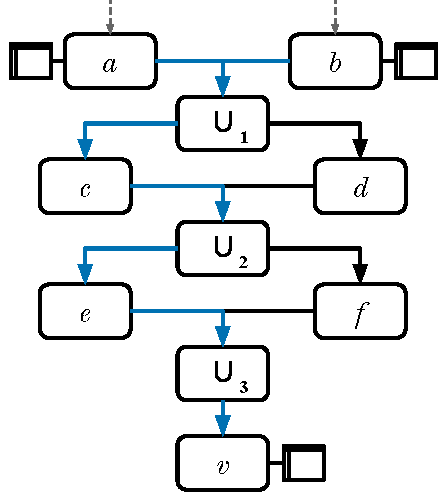
\includegraphics{diagrams/Chained Unions.pdf}
  \caption{Chained unions. Only nodes $a$, $b$, and $v$ hold state. Highlighted
  in \textbf{\color{set1}blue} are two upquery paths that $\cup_1$ must combine
  upquery responses for.}
  \label{f:chained-union}
\end{figure}

Figure~\ref{f:chained-union} shows a dataflow segment where the precise grouping
mechanism is important (\texttt{upquery\_path\_group} in the code listing).
There are three unions in a chain, which makes eight distinct upquery paths. If
$v$ encounters missing state, it must therefore issue eight upqueries, one for
each path. $a$ and $b$ both appear as the root of four paths, and will be
upqueried that many times. The issue arises at the unions, which need to do
the aforementioned union buffering.

Ultimately, a single upquery response must reach $v$. This means that $\cup_3$
must receive two upquery responses, one from $e$ and one from $f$, which it must
then combine. So $\cup_2$ must \emph{produce} two upquery responses, one
destined for $e$ and one for $f$. This in turn means that $\cup_2$ must receive
two upquery responses from $c$, and two from $d$. Which again means that
$\cup_1$ must produce four responses, two for $c$ and two for $d$, out of the
eight responses it receives (four from $a$ and four from $b$).

These are all the upqueries that pass through $\cup_1$:
        
\begin{multicols}{4}
\begin{description}
  \item [1.] $a\,\to\,c\,\to\,e$
  \item [2.] $a\,\to\,c\,\to\,f$
  \item [3.] $a\,\to\,d\,\to\,e$
  \item [4.] $a\,\to\,d\,\to\,f$
  \item [5.] $b\,\to\,c\,\to\,e$
  \item [6.] $b\,\to\,c\,\to\,f$
  \item [7.] $b\,\to\,d\,\to\,e$
  \item [8.] $b\,\to\,d\,\to\,f$
\end{description}
\end{multicols}

$\cup_1$ must combine these so that each downstream union receives the responses
that they expect from their inputs. This grouping achieves that:

\begin{multicols}{2}
\begin{description}
  \item [1/5.] $a/b\,\to\,c\,\to\,e$
  \item [2/6.] $a/b\,\to\,c\,\to\,f$
  \item [3/7.] $a/b\,\to\,d\,\to\,e$
  \item [4/8.] $a/b\,\to\,d\,\to\,f$
\end{description}
\end{multicols}

The key observation is that the distinction between $a$ and $b$ does not matter
downstream of $\cup_1$; a delta that arrived from $a$ is indistinguishable from
one that arrived from $b$. Similarly, the distinction between $c$ and $d$ no
longer matters past $\cup_2$, and the same for $e$ and $f$ past $\cup_3$.
\texttt{upquery\_path\_group} is thus defined as a unique identifier for $v$'s
upquery plan plus the sequence of nodes between the union and the target of the
upquery response.

\subsection{Joins}

Upqueries across unions must go to all the ancestors. But across joins,
upqueries must only go to \textbf{one} ancestor. This is because a join that
processes a message from one ancestor already queries the ``other'' ancestor and
pulls in relevant state from there. If both sides were queried, the processing
of the upquery responses at the join would produce duplicates of every record.

Noria supports two types of joins: inner joins and partial outer joins (i.e.
``left'' and ``right'' joins). For an inner join, either ancestor can be the
target of the upquery, whereas for a partial outer join, the upquery \emph{must}
go to the ``full'' side\,---\,the side from which all rows are
yielded\footnote{An upquery for a column that originates from the non-full
ancestor must be routed according to its value. If it is \texttt{NULL}, the
upquery must go to the left, with additional later filtering, whereas if it is
non-\texttt{NULL}, it can go to the non-full side without issue. Noria does not
support such upqueries.}. Otherwise, the upquery may produce only a subset of
the results for the join.

\subsubsection{Dependent Upqueries}

Since upqueries travel through only one ancestor of a join, joins do not need to
buffer upquery responses the same way unions do. However, when a upquery
response passes through a join operator, the join does perform lookups into the
state of the other side of the join. With partial state, those lookups may
themselves encounter missing entries. When this happens, a problem arises: Noria
\emph{must} produce an downstream upquery response because the application is
waiting for it, but cannot produce that response since required state is
missing.

For the purposes of exposition, and without loss of generality, the text below
refers to the join ancestor that was upqueried as the left side, and the
ancestor that a lookup missed in as the right side.

The join must issue an upquery to the right hand side for the state that is
missing to complete the processing of the original upquery response from the
left. However, this \textit{dependent upquery} may take some time to complete,
and the system must decide what to do in the meantime. Recall that the join is
still in the middle of processing an upquery response.

An obvious, but flawed strategy is to have the join block until the response
arrives. This would not only stall processing of deltas from the left parent,
but also leads to a deadlock. In order to observe the eventual upquery response,
the join's domain must continue to process incoming messages to the right parent
(\S\ref{s:join-state-dupe}). But in doing so, it may encounter a different
upquery response from the right parent. That upquery response may require a
lookup into the left parent's state, which may itself encounter missing entries.
The join is then forced to block on both inputs perpetually.

Instead, the join \emph{discards} the current upquery response, and remembers
the upquery parameters that triggered it, and the missing state that must be
filled. It then continues processing the next update as normal. When the missing
entries are eventually filled, Noria \emph{re-issues} the original upquery to
the join's left parent using the saved parameters. This time, all entries
required for the lookups into the right-hand parent's state are present, and the
downstream upquery response can be produced. As far as the downstream dataflow
is concerned, nothing abnormal has happened\,---\,the upquery response just took
longer to arrive.

\subsubsection{Incongruent Joins}
\label{join-evictions}

As discussed in \S\ref{s:partial:linear}, if some key $k$ is present in a
materialization $m$, it is also present at every materialization above $m$ from
the upquery chain that ultimately produced the entry for $k$ in $m$. However,
certain query graphs produce dataflow where more than one key is used to compute
an entry. Consider a dataflow that joins two inputs, \texttt{story} and
\texttt{user}, on the story's author field. A downstream operator issues an
upquery for story number 7. The upquery is issued to \texttt{story}, which
produces a message that contains story number 7 with author ``Elena''. That
message arrives at the join, which issues a dependent upquery to \texttt{user}
for ``Elena''. When that dependent upquery resolves, the join produces the final
upquery response, and the state for story number 7 is populated in the
downstream materialization.

Next, an editor changes the author for story number 7 to ``Talia''. This
takes the form of a delta with a negative multiplicity record for \texttt{[7,
"Elena"]} and a positive one for \texttt{[7, "Talia"]}. When this delta arrives
at the join, it may now miss when performing the lookup for ``Talia''. According
to the partial model so far, the join should drop \texttt{[7, "Talia"]}, and
only allow the negative for ``Elena'' to propagate to the downstream
materialization. But this violates Invariant~\ref{i:missing-suffix}, since there
exists downstream state that reflects the discarded update. And indeed, when
this happens, the state for article number 7 becomes empty (though not missing),
and any subsequent read for article number 7 receives an empty response, which
violates Invariant~\ref{i:no-holes}.

What happened here was that the entry for key $k$ in the leaf-most
materialization depends not only on state entries indexed by the same $k$
upstream, but also on state entries indexed by other keys upstream. While $k$
must be present upstream, no such guarantee exists for other keys.

This is a result of \textit{incongruent joins}; joins whose join column is not
the same as the downstream key column. Incongruence is determined with respect
to each upquery path that flow through a join. In the case above, the author
join is incongruent with an upquery on the story number column, since the join
column is the author column. However, the join is congruent with upqueries from
a hypothetical downstream view that is keyed by author instead. A join that is
incongruent with any upquery path that flows through it is considered an
incongruent join.

Noria can easily recognize incongruent joins through key provenance
analysis\,---\,if an upquery flows through a join, and the upquery column is not
the same as the join column, the join is incongruent. If an incongruent join
encounters missing state while processing a delta at runtime, it must take
action to ensure that downstream state remains correct. Since the domain that
processes the join cannot produce a valid delta, and does not know what state is
present and missing in the downstream dataflow, its only option is to issue an
eviction for any downstream state that \emph{may} be rendered stale. Concretely,
if an incongruent join processes a record $r$ and encounters a missing state
entry, it should issue an eviction downstream on all incongruent upquery paths
using the appropriate values from $r$. For example, if the join column is $c_j$,
and upquery path $u_i$ through the join is keyed by column $c_i$, then the join
should issue downstream evictions of $r[c_i]$ for each $u_i$ where $c_i \neq
c_j$.

\paragraph{All Together Now.}
%
With unions and joins covered, the argument is complete. In all dataflows that
Noria can construct, no matter how they diverge and merge, the outlined
mechanisms ensure that the system invariants are maintained at every node, and
thus in Noria as a whole.

\section{Sharding}
\label{s:challenge:sharding}

Noria supports sharding cliques of operators to add parallelism to particular
sections of the dataflow (\S\ref{s:noria:sharding}). When Noria decides to shard
operators in this way, upqueries must continue to work. Partial state with
sharding mainly follows the rules of partial across unions
(\S\ref{s:upqueries:union}), with three changes:

First, if the node that receives the upquery, R, is sharded the same way as the
querying node, Q, the upquery is sent \emph{only} to the same shard of R as the
one that is querying. This is called a \textit{narrow} upquery, and avoids
queries to shards that hold no relevant data. This rule applies even if the
upquery key differs from the sharding key, since while other shards may have
relevant data, that data would be discarded before reaching the current node
anyway. Noria decides whether upqueries should be narrow or broad when it
determines an operator's upquery plan\,---\,key provenance provides sufficient
information to make the decision.

Second, when a narrow upquery response reaches the \emph{first} shard merger
(effectively a union across shards) on its path, the response must not be
buffered, unlike other upquery responses across unions. This is because
the other upstream shards will not be sending responses.

Third, when the upquery response for an upquery that originated at a sharded
node reaches the \emph{last} sharder on its path, that sharder must direct that
response only to the querying shard. This is equivalent to the general rule that
upquery responses only flow along the edges that the upquery traversed. The
upquery that triggered the response did not touch other shards of the upquery
originator, and so the response should not go there.

Beyond those three modifications, the existing logic for handling upqueries
across forked strands of dataflow is sufficient.

% \footnote{Since shard mergers have only one operator (but many shards) as their
% ancestor, they use the shard index of the operator that sent each input as a way
% to distinguish between input paths, rather than the index of the operator
% itself. Otherwise, they operate entirely as a union.}


\chapter{Implementation}
\label{s:impl}

The prototype implementation of Noria with partial state consists of 65k lines
of Rust. It can operate on a single server or across a cluster of servers.

The source code is available at \url{https://github.com/mit-pdos/noria}.

\paragraph{Interface.}
Applications interface with Noria either through native Rust bindings, using
JSON over HTTP, or through a MySQL adapter~\cite{noria-mysql}.

\paragraph{Storage.}
The implementation maintains views in memory, and can maintain base tables
either in memory (the default) or on disk using using RocksDB~\cite{rocksdb}, a
key-value store based on log-structured merge trees.

\paragraph{Missing State.}
Noria does not store markers (``tombstones'') for missing results in a
materialization. Instead, it stores materialized results that are known to be
empty in hash tables alongside other (non-empty) materialized results. This
allows even empty results to be evicted to save space.

\paragraph{Upquery Bypass.}
When Noria encounters missing state and issues an upquery, it sends that
upquery directly to the root of the upquery path. This saves sending the
message along internal edges, but does not affect correctness as the
intermediate operators only forward the upquery upstream.

\paragraph{Batching.}
Noria uses several time-limited batching buffers to improve performance. Writes
to a base table are buffered for a few microseconds, and are emitted into the
dataflow as a single combined update to amortize lookup and processing costs at
operators like aggregations and joins. Noria also buffers upqueries in case
other misses for different keys along the same upquery path occur in quick
succession, and forwards them in a single batch.

\paragraph{Runtime.}
To multiplex I/O and compute, Noria uses Tokio~\cite{tokio}, a high-performance
asynchronous Rust runtime. Tokio manages a pool of threads that cooperatively
schedule thread domain processing (\S\ref{s:noria:partitioning}), query
handling, and control operations like adding and removing queries.

\paragraph{Network Protocol.}
Noria uses a very simple, Rust-specific binary encoding for its network
protocol. The protocol tags each request and response with a required
identifier, which allows Noria to respond to requests as they complete on the
server, rather than process them one-at-a-time. This also enables the Noria
dataflow to process updates in batch more often, since multiple client requests
can be batched together.

\paragraph{Running Out of Memory.}
Noria has no special mechanisms for monitoring its own memory use. If eviction
is not aggressive enough, or a given materialization simply requires more memory
than is available, the Noria process crashes.

\paragraph{Storing Result Sets.}
Noria stores materialized views as a hash table whose key is the view's
parameter column. The value for a given entry in the hash table is the
collection of rows that a query with that entry's key should return. There
may be many rows for a given key, including duplicates, so to support efficient
removal of individual rows, the result set is stored as a hash bag: a hash table
where the index is each distinct row, and the value is that row's multiplicity.

\paragraph{Resizing Pauses.}
Many of the benchmarks in this thesis continuously accumulate more data,
especially in the base tables, and then measure latency over time. Since the
benchmarking harness captures the full distribution of latencies, including the
far tail, this surfaced a number of ``amortized'' costs from data structures
like hash tables and vectors that occasionally double in size as they grow.
Those resizes caused significant spikes in tail latency, which was unfortunate
in experiments that aimed to measure tail latency specifically. Noria therefore
now uses specialized data structures whose resize behavior is \emph{also}
amortized by spreading the cost of resizes across multiple later inserts.

\paragraph{Nagle's algorithm.} Disabled, as it should be for anything
latency-sensitive. Many hours were lost in the searches for TCP sockets where it
had not yet been disabled.

\paragraph{Fast Reads.}
Query handlers process clients' RPCs to read from external views. They must
access the view with low latency and high concurrency, even while a thread
domain applies updates to the view. To minimize synchronization, Noria uses
double-buffered hash tables for external views that are wait-free for
readers~\cite{evmap}: the thread domain updates one table while read handlers
read the other, and an atomic pointer swap exposes new writes. This design can
significantly improve read throughput on multi-core servers over a
single-buffered hash table with bucket-level locks in workloads with high skew.
Internally, the design resembles the ``left-right'' concurrency
scheme~\cite{left-right}.

\paragraph{Operator Implementation.}
The implementation of the various relational operators in Noria is perhaps
surprisingly straightforward, despite the vast literature on how to implement
joins and aggregations more efficiently. The primary reason for this is that the
operators must work in an incremental fashion with small batches of rows
arriving intermittently. Most intelligent implementations play tricks with how
they arrange and walk the indices of upstream tables, and how the columns of the
output rows are collected, but this is not feasible in a tuple-at-a-time system
like Noria. Nevertheless, the operators try to be efficient where possible: they
only look up each distinct value of a join key or aggregation group column in a
batch of rows once, and sort batches before processing to improve cache
efficiency.

\paragraph{Query-Through.}
The restriction that join inputs must be materialized
(\S\ref{s:join-state-dupe}) is not quite as strict in practice as it might first
seem. The true requirement is that the source of the join lookups must reside in
the same thread domain, not that the join's \emph{immediate} ancestors be
materialized. For example, if an aggregation (which must have its output
materialized) is a followed by a filter, which is then followed by a join, the
output of the filter does not \emph{also} need to materialized if all nodes are
in the same thread domain. Noria can reuse the aggregation's materialization as
long as the filter is applied to any lookup results before the join sees them.


\chapter{Evaluation}
\label{s:eval}

This thesis is built on the belief that view materialization is useful, but
prohibitively costly to use with current solutions. It presents partial state as
a solution to this problem that allows retaining the benefits of view
materialization at a fraction of the cost. Section \ref{s:eval:why} evaluates
the validity of this assumption, and the efficacy of partial state as a
solution.

Existing application deployments tend to implement their own ad-hoc caching
logic, usually by placing a dedicated cache in front of the database. Some
larger companies have also built comprehensive tooling to manage their caches
correctly. Section \ref{s:eval:alts} looks at how Noria serves as an attractive
alternative to these approaches.

With partial state, only a subset of each view is materialized, and missing
results are computed on-demand. Partial state thus presents a trade-off between
memory use (cache size) and tail latency (miss rate). Section \ref{s:eval:cost}
explores the effects of this trade-off.

Developers may be hesitant to switch applications that already use a cache today
to Noria without some evidence that their performance won't regress.
Unfortunately, the impact Noria would have on any given application is highly
dependent on the particulars of each application, and is thus hard to measure.
To demonstrate that Noria can offer comparable absolute performance to existing
caching solutions, section \ref{s:eval:kvperf} compares Noria lookup performance
to that of Redis under ideal caching conditions.

An added benefit of partial state is that it allows applications to introduce
new queries/views without materializing it entirely up-front. This enables fast
adoption of new queries, but also means that queries to new views are initially
slow. Section \ref{s:eval:mig} evaluates these partial state migrations compared
to traditional all-at-once materialization.

The ability of partial state to reduce the memory use of view materialization
depends on skew in the application's data and access patterns. It allows Noria
to reduce latency for a significant fraction of requests by keeping only a few
results cached. While it is impossible to predict the skew for an arbitrary
application's data and queries, section \ref{s:eval:patterns} gives a simplified
theoretical model to help with estimation.

\section{Experimental Setup}
\label{s:eval:setup}

The experiments in this chapter primarily use the Lobsters news
aggregator web application at \url{https://lobste.rs}~\cite{lobsters}. This
application was chosen because it is open-source (so we can see what queries it
issues), because it resembles many larger-scale applications (like Hacker News
or Reddit), and because statistics about the site's data and access patterns are
available~\cite{lobsters-data}.

The evaluation uses a workload generator that issues page requests
according to the available statistics~\cite{generator}. It does not run the
real Lobsters Ruby-on-Rails application, as it is prohibitively slow. Instead,
all experiments use an adapter that turns page requests directly into the
queries the real Lobsters code would issue for that same page request. The
generator supports scaling up the rate of access and user count to emulate a
larger user base for benchmarking.

\begin{figure}
  \begin{tabular}{ p{0.8in} | r | r | r | p{2.9in} }
    Page & \% & W & Q & Description \\
    \hline
    Story & 55.8 & 1 & 14 & Renders an individual story's page, including its
    popularity score, comments, and the scores of its comments.\\
    Frontpage & 30.1 & 0 & 14 & Lists the 25 most highly scored stories, along
    with their authors and scores.\\
    User & 6.7 & 0 & 7 & Renders a user summary page, including what story
    ``tags'' they contribute to.\\
    Comments & 4.7 & 0 & 9 & Like the frontpage, but for comments.\\
    Recent & 1.0 & 0 & 14 & 25 most recently added stories, along with their
    authors and scores.\\
    Vote & 1.2 & 1 & 2 & Vote up/down a given comment or story.\\
    Comment & 0.4 & 2 & 5 & Add a new comment to a story.\\
  \end{tabular}
  \caption{Pages in Lobsters. \% indicates the percentage of requests that load
  the given page. W is the number of writes loading the page requires, and Q is
  the number of queries it issues.}
  \label{t:lobsters-pages}
\end{figure}

The various pages in Lobsters differ significantly in what queries they issue,
how many queries they issue, and the extent to which they are read or write
heavy. Table~\ref{t:lobsters-pages} gives an overview of the frequency of
requests for each page, what loading the page entails, and a brief description
of that page. In all evaluation results, latency is measured across all
requests, no matter what page they are for.

Experiments run on Amazon EC2 r5n.4xlarge instances, which have 16 vCPUs and
128GB of memory. The server is always given a dedicated host, while
load-generating clients are split across one or more m5n.4xlarge instances
depending on the desired load factor.

The benchmarks are all ``partially open-loop''~\cite{frank-open-loop}:
clients generate load according to a workload-dictated distribution of
interarrival-times, and has a limited number of backend requests outstanding,
queueing additional requests. This ensures that clients maintain the measurement
frequency even during periods of high latency. The test harness measures offered
request throughput and ``sojourn time''~\cite{open-loop-cautionary-tale}, which
is the delay the client experiences from request generation until a response
returns from the backend.

All experiments measure memory use using the resident virtual memory of the
server process (VmRSS). This measurement therefore includes all indexes, runtime
allocations, and other bookkeeping metadata. For Noria, it also includes the
data stored in the base tables.

Since the benchmarks introduce more data as they run, memory use increases over
the course of each run. Experiments are run for a bit over 5 minutes unless
otherwise specified, and memory measurements are taken at the end of the run.

\begin{inprogress}
  Note about stability of experimental results once all experiments are nailed
  down.
\end{inprogress}

\section{Benefits and Costs of View Materialization}
\label{s:eval:why}

The core argument of this thesis is that partial state makes view
materialization feasible. Bundled up in that argument are several intertwined
questions that must be answered before further evaluation of partial state is
interesting:

\begin{enumerate}
    \item Why is view materialization desirable?
    \item Why is view materialization not feasible currently?
    \item Does partial state improve on this situation?
\end{enumerate}

\begin{figure}[h]
  \centering
  \includegraphics{graphs/lobsters-throughput.pdf}
  \caption{Maximum achieved throughput on Lobsters benchmark with and without
  view materialization. Without view materialization, MySQL must compute query
  results each time. Traditional (full) view materialization runs out of memory
  at $\approx$4.6k pages/second. Partial state allows Noria to reduce memory use
  significantly so that it can achieve higher throughput.}
  \label{f:lobsters-throughput}
\end{figure}

Figure~\ref{f:lobsters-throughput} attempts to explain why view materialization
is desirable. It compares the highest sustainable request load of three
different systems: MySQL, Noria without partial state, and Noria with partial
state. MySQL is run entirely in RAM by running it on a ramdisk, and on its
lowest isolation level. The figure shows the highest Lobsters throughput each
system achieves before its mean latency exceeds 50ms.

View materialization alone (as provided by Noria) improves performance by almost
$12\times$ compared to MySQL, as query results are now frequently cached.
However, without partial state, this performance increase comes at a significant
memory cost. Beyond 4.6k pages/second, it runs out of memory, and cannot
support the workload. With partial state, Noria uses much less memory at a given
load factor, which allows it to support 67\% higher throughput, almost
20$\times$ that of MySQL%
\footnote{The Noria benchmarks are memory constrained, not CPU constrained.
MySQL fully loads all 16 cores at 391 pages per second.}.

\begin{figure}[h]
  \centering
  \includegraphics{graphs/lobsters-memory.pdf}
  \caption{Memory use two minutes into the Lobsters benchmark at 4.6k pages per
  second. Striped bars store base tables on disk using RocksDB.}
  \label{f:lobsters-memory}
\end{figure}

Figure~\ref{f:lobsters-memory} shows the memory use at 4.6k pages per second
with and without partial state. It demonstrates both the issues with full
materialization, and the improvements brought about by partial state. With full
materialization, Noria must store every result for every query in memory. In
contrast, with partial state, Noria stores only frequently accessed results,
which cuts memory use in half.

The memory use reductions with partial state are a direct result of the skew in
Lobsters data popularity and access patterns. Many pages are simply never
visited over the course of the benchmark, and so need not be brought into the
cache. With partial state, Noria also evicts infrequently accessed results,
which further reduces memory use, and ensures that the cache does not eventually
grow to contain all results.

\begin{figure}[h]
  \centering
  \includegraphics{graphs/lobsters-opmem.pdf}
  \caption{Estimated operator state data size two minutes into the Lobsters
  benchmark at 4.6k pages per second. The value indicated includes only the sum
  total size of rows in each operator's state, not data structure overheads,
  indices over the data, or other memory allocations. Base tables are not
  included.}
  \label{f:lobsters-opmem}
\end{figure}

Much of Noria's memory use goes to storing the base tables in memory. Since
partial state cannot evict base table state, this limits how much memory can
potentially be saved. The figure therefore also includes memory use when running
Noria with its durable RocksDB storage backend for base tables. In that
configuration, base tables are kept on disk, not in memory, which makes the
memory savings from partial state more apparent\,---\,the memory use is now
about a third that without partial state.

Various other runtime overheads that partial state cannot eliminate remain, such
as data structure overheads, and allocations for in-flight requests and pending
responses. With diligent memory optimization, this overhead could likely be
further reduced to increase the relative benefits from partial state. To provide
some insight into how far memory use can be reduced,
Figure~\ref{f:lobsters-opmem} shows the total size of the data contained in all
non-base operator state in Lobsters. This metric measures \emph{only} the sum of
the data in each row, and excludes all other memory overheads, such as hash
tables, additional indices, or allocations elsewhere in the application. The
results indicate that partial state in isolation requires only 1.5\% of the
total operator state to be materialized; significantly less than the
$\sfrac{1}{3}$ seen in Figure~\ref{f:lobsters-memory}. This suggests that there
is further potential for reducing partial state's memory footprint.

Since partial state uses less memory, applications that do not need higher
throughput can instead reduce cost by using hosts with less memory. For example,
on AWS EC2, going from a 64GB instance type with 16 cores (\texttt{m5n.4xlarge})
to a 128GB instance type with 16 cores (\texttt{r5n.4xlarge}) comes at a 25\%
price increase. Instances with 256GB of memory only come with 32 cores
(\texttt{r5n.8xlarge}) or more, and come out at twice the price of 128GB.

\section{Rolling Your Own}
\label{s:eval:alts}

Many applications already require lower latency and higher throughput than
straightforward SQL queries against traditional relational databases provide.
Developers often implement manual optimizations to improve their application
performance, and introduce additional complexity into their applications in the
process. These optimizations usually come in one of two forms: denormalization
and caching. This section discusses each of these optimization techniques in
turn, as well as how Noria makes them unnecessary.

\subsection{Denormalization}

The relational database model~\cite{relational} encourages developers to use
``normalized'' schema in which redundant data%
\footnote{The relational model differentiates between strongly and weakly
redundant data\,---\,``redundant'' here refers to strong redundancy.}
that can be derived from other data is not stored. Instead, the model suggests
that derived or computed data be produced on-demand using relational operators
like joins and aggregations. The original paper then adds:

\begin{quote}
Only in an environment with a heavy load of queries relative to other kinds
of interaction with the data bank would strong redundancy be justified in the
stored set of relations.
\end{quote}

As discussed in the motivation section for this thesis, many web applications
fall into exactly this category. Queries are far more common than inserts or
updates, and with a normalized schema they must constantly expend resources to
re-compute such derived data. For this reason, web developers often explicitly
denormalize their schema to include data that would be prohibitively expensive
to compute on-demand.

For example, in Lobsters, each story has a ``hotness'': a score of how popular a
story is, and thus how far up it should appear in listings. This value depends
on a lot of parameters, such as the number of votes, the number of comments,
etc. It would be prohibitively expensive to compute a story's hotness directly
in the queries, especially in the context of computing the front page view,
which requires the hotness for \emph{all} stories to rank them. Instead, the
Lobsters developers add a computed column, \texttt{hotness}, to the
\texttt{story} table. This column is then updated whenever relevant data
changes, such as when:

\begin{itemize}
    \item a story is upvoted or downvoted.
    \item a comment is added to a story.
    \item a comment on a story is upvoted or downvoted.
    \item a comment or vote is deleted.
    \item one story is merged into another.
\end{itemize}

There are several such computed columns in Lobsters. For each one, developers
must inspect all write paths, and change them to ensure that they correctly
update all related computed values. This process is manual and error-prone, but
also necessary: without these manual optimizations, Lobsters running against
MySQL cannot keep up with even a single request per second.

With Noria, such manual denormalization is unnecessary. View materialization
automatically stores and maintains derived data so that it is efficient to
query. The developer can continue to use normalized schemas and queries, and
does not need to modify their application code to manage denormalized columns
and tables.

\subsection{Caching}

If denormalization does not sufficiently improve the application's performance,
the next step is usually to add a cache in front of the database. This cache
often takes the form of a key-value store, like Redis or Memcache, which holds
frequently accessed, computed results. When the application issues a query, it
checks the (fast) cache first, and only if the results are not available in
cache is the (slower) backend consulted.

A dedicated cache speeds up reads that hit, but introduces significant
application complexity. Just like for manual denormalization, all parts of the
application that modify data related to any given cache entry must know to also
invalidate or update the cache. In addition, the developers must ensure
that if multiple clients miss on a given entry, they do not hit the backend
database all at once. This is especially important if a popular entry is
invalidated, as it may cause a ``thundering herd'' effect where a large number
of clients swarm the backend and overwhelm it. Furthermore, since the clients
must now access two separate systems, mechanisms must be in place to ensure that
the cache remains consistent with the underlying data. This is difficult since
data may be updated at any time, including just after a client has fetched the
(then) latest data from the database to update the cache.

Because of the challenges above, implementing caching ``correctly'' requires
highly sophisticated machinery~\cite{facebook-memcache, transactional-cache,
orm-cache, sql-cache}, which developers may not even think to employ. A survey
from 2016 found that 0.3-3.0\% of application code spread across 2.1-10.8\% of
the application's source files is caching-related, and that cache-related issues
make up 1-5\% of all issues~\cite{caching-is-hard}.

With Noria, there is no need to maintain such a query result cache, as Noria's
in-memory materialized views provide high-throughput, low-latency queries
directly from the database. Thanks to partial state, Noria's materialized views
are usable even for applications whose full cache state exceeds the amount of
memory available on the server host. Since Noria automatically maintains the
materialized views, the application also does not need code to manage cache
invalidation or to address challenges like thundering herds.

\section{The Memory/Latency Trade-off}
\label{s:eval:cost}

Partial state's main drawback compared to complete materialized views is
that the results for an application's query may not be known. Or, stated
differently, some reads may miss. When this happens, the system must upquery the
missing state, which takes time and consumes resources otherwise dedicated to
writes. This shows up as increased tail latency for the application: queries
whose results are not known must wait to be computed. The hope with partial
state is that, once the commonly-accessed query results are cached, latency
quickly drops such that going forward only infrequently accessed query results
must be computed on-demand.

\subsection{Warming the Cache}

\begin{figure}[t]
  \centering
  \includegraphics{graphs/lobsters-timeline.pdf}
  \caption{Lobsters latency timeline at 1.5k pages per second across all pages
  with eviction. Figure shows the latency profile seen by the client over time,
  starting at the point when the first query is issued. Time increases along the
  x-axis, with each bin sampling twice as long as the previous one. The measured
  latency for each time bin is plotted on a logarithmic scale on the y-axis.
  Progressively lighter colors include more of the tail.}
  \label{f:lobsters-timeline}
\end{figure}

The cost of these misses is particularly visible when Noria starts with empty
state. This is equivalent to starting a more traditional caching system with an
empty (cold) cache, and having to ``warm'' it by filling in the most popular
entries. To measure this warming period, Figure~\ref{f:lobsters-timeline} shows
the latency profile seen by the Lobsters benchmark described in
\S\ref{s:eval:setup} over time, starting at the point when the first query is
issued. Time increases along the x-axis, and the measured latency for each time
bin is plotted on a logarithmic scale on the y-axis. Progressively lighter
colors indicate values further into the tail.

The figure shows that latency is initially high, but after a few seconds, the
mean and 95th percentile latency drop below 10 milliseconds. By the time a
minute has passed, the 99th percentile has followed suit. Since only a small
portion of the total computed state is cached (as shown in
Figure~\ref{f:lobsters-memory}), this supports the hypothesis that partial state
achieves low latency once the most commonly accessed results are cached.
The latency is primarily determined by the number of queries each page issues,
as each one requires a round-trip to Noria.

\subsection{Impact on Tail Latency}

\begin{figure}[h]
  \centering
  \includegraphics{graphs/lobsters-memlimit-cdf.pdf}
  \caption{CDF of sojourn latency across all Lobsters pages at 1.5k pages per
  second with decreasing permitted memory use. The figure depicts steady-state
  operation\,---\,the benchmark has been allowed to run for two minutes before
  the latency is measured.}
  \label{f:lobsters-mem-latency}
\end{figure}

Partial's trade-off is that of memory use versus tail latency; as you allocate
less memory to Noria, less of your tail can be pre-computed, and thus more of
your requests will be slow as it must be computed on-demand.
Figure~\ref{f:lobsters-mem-latency} shows this trade-off in the steady state%
\footnote{The benchmark runs for two minutes before latencies are sampled.}
of the application. It plots the CDF of the sojourn latency across all requests
with increasingly aggressive eviction. As Noria is asked to
reduce memory use by evicting more aggressively (darker purple lines), more
requests take longer, and the tail grows. In other words, the further you want
to reduce memory use, the more you pay in latency. Without partial
materialization, you do not have this choice\,---\,requests in the tail will
always be fast, but only as long as all the materialized views fit in memory.

\begin{figure}[h]
  \centering
  \includegraphics{graphs/lobsters-durability-cdf.pdf}
  \caption{CDF of sojourn latency across all Lobsters pages at 1.5k pages per
  second with base tables in memory and on disk. The figure depicts steady-state
  operation\,---\,the benchmark has been allowed to run for two minutes before
  the latency is measured.}
  \label{f:lobsters-dur-latency}
\end{figure}

If base tables are not kept in memory, the cost of recomputing missing state
from the data in those base tables increases. Exactly how much depends on the
performance characteristics of the durability backend in use.
Figure~\ref{f:lobsters-dur-latency} shows a CDF of page latencies when Noria's
RocksDB backend is used, with writes going to a ramdisk. Latencies increase by
anywhere from 20-50\%, depending on the number of misses a given page request
experiences.

The reason why the whole curve shifts, rather than just the tail, is that these
CDFs are across \emph{all} the different page types in Lobsters. Each one issues
a different set of queries, and so their total time differs, as does the effect
of a longer tail. The exact shape of this curve, and how it shifts in response
to varying resources, depends on the application in question.

% \begin{inprogress}
% Full materialization is slightly faster than partial materialization because
% SOMETHING SOMETHING either join eviction or faster lookups due to no tombstones?
% \end{inprogress}

\subsection{Memory Use and Throughput}

Memory use can only be reduced so far before the system no longer keeps up with
the offered load. If some of the most frequently accessed (``hot'') query
results are not cached, the system will constantly have to re-compute those
results to satisfy reads that come in shortly after that query result is
evicted. This cache churn increases latency and decreases throughput, often
significantly. Essentially, the system will never finish warming the cache, and
latency will remain at the high levels shown early in
Figure~\ref{f:lobsters-timeline}. For Lobsters, this happens around the 18GB
mark. If the eviction is tuned to be more aggressive than that, Noria can no
longer sustain 1.5k pages per second.

Generally speaking, as throughput increases, so must the memory budget. The
intuition behind this is that the memory budget effectively dictates your hit
rate. The more requests are issued per second, the more misses (in absolute
terms) result from a given hit rate. If those misses in the tail are
distinct, Noria must satisfy \textbf{more} upqueries as load increases, while
also handling that added load.

\begin{listing}[h]
  \begin{minted}{sql}
    SELECT articles.*, COUNT(votes.user_id)
    FROM articles
    LEFT JOIN votes ON (articles.id = votes.article_id)
    GROUP BY articles.id
    WHERE articles.id = ?
  \end{minted}
  \caption{Simplified query for vote counting in Lobsters.}
  \label{l:votes}
\end{listing}

While this correlation between throughput and memory use exists in Lobsters, it
is difficult to show clearly as each page issues many different queries, and
overall load is relatively low. For this reason, the next set of benchmarks use
a simplified version of one particular query from Lobsters shown in
Listing~\ref{l:votes}. It counts the number of votes for an article, and
presents that alongside the article information. The benchmark issues requests
distributed as 99\% reads and 1\% writes (inserts into \texttt{votes}). The
access pattern is skewed such that 90\% of requests access 1\% of keys across
10M articles%
\footnote{The benchmark samples keys from a Zipfian distribution with a skew
factor ($\alpha$) of 1.15}. Load is generated by four clients, and each one
batches requests for a maximum of 10ms to reduce serialization overheads.

\begin{figure}[h]
  \centering
  \includegraphics{graphs/vote-throughput-memlimit.pdf}
  \caption{Achieved throughput vs 95th percentile request latency in vote with
  increasingly aggressive eviction. Offered load increases along the points on
  each line. A near-vertical line indicates that the system no longer keeps up
  with offered load.}
  \label{f:vote-throughput-memlimit}
\end{figure}

Figure~\ref{f:vote-throughput-memlimit} demonstrates the connection between
throughput and memory use. It shows throughput-latency lines for the vote
benchmark with progressively more aggressive eviction. Each point along each
line is a higher offered load; its x-coordinate is the achieved throughput, and
its y-coordinate is the measured median latency. When Noria no longer keeps up,
you see a ``hockey stick'' effect, where achieved throughput no longer
increases, while latency spikes.

The figure shows that as the offered load increases, Noria needs to use more
memory to keep up. If we do not bound memory use, Noria can keep up with higher
load at the cost of caching most of the dataset (about two thirds).

\section{Absolute Cache Performance}
\label{s:eval:kvperf}

Despite how error-prone the approach is, ad-hoc, per-application caching is
still common in practice. And while Noria eliminates most of the developer
burden of getting caching right, it must offer competitive performance with
manually constructed caching solutions to present a viable alternative.

Unfortunately, this is difficult to evaluate, since high-performance solutions
are often developed specifically for a given application, and not available as
general-purpose tools. And effectively applying the general-purpose tools that
\textbf{are} available, like memcache and Redis, requires significant effort on
the part of the application authors (or the evaluators). To manually add caching
support to Lobsters' ~80 queries, including thundering herd mitigation and
incremental updates, would be a significant undertaking.

This fact alone is, in essence, an argument for the Noria approach. The manual
effort involved in making Lobsters use Noria is minimal\,---\,just switch the
code to query Noria instead of MySQL, and you get automatic caching. In many
cases the application code can even be simplified, such as by removing manual
materialization decisions like the story ``hotness'' column described in
\S\ref{s:eval:alts}.

Nevertheless, an experiment to evaluate Noria's absolute performance compared to
a ``real'' cache is necessary. Without such a comparison, Noria can only claim
to be ``faster than MySQL'', but not ``as fast as a cache''.

The next experiment runs the vote benchmark from Listing~\ref{l:votes} against
Redis~\cite{redis}, a popular high-performance key-value store that is commonly
used as a caching backend. In an attempt to approximate how a carefully planned
and optimized application caching deployment might perform, it makes the
following modifications to the benchmark:

\begin{itemize}
 \item Every access hits in cache, to emulate perfect thundering herd mitigation
   and invalidation-avoidance schemes.
 \item Nearly all accesses (99.99\%) are reads, since writes would be
   bottlenecked by the backing store.
 \item Data is not stored anywhere except Redis.
 \item Accesses are batched to reduce serialization cost and increase
   throughput. Specifically, reads are \texttt{MGET}s, and writes are pipelined
    \texttt{INCRBY}s.
\end{itemize}

This is not a realistic use of Redis as a cache, and ignores the complexities of
integrating the cache with the application. It also assumes that cached query
results are never spread across more than one key in the cache. However, it
enables an evaluation that assumes the best about the underlying caching
strategy and system.

\begin{figure}[h]
  \centering
  \includegraphics{graphs/vote-redis.pdf}
  \caption{Achieved throughput vs 95th \%-ile request latency in cache-optimized
  vote. Offered load increases along the points on each line. The vertical
  line indicates $16\times$ the highest Redis throughput, since Redis is
  single-threaded.}
  \label{f:vote-redis}
\end{figure}

Figure~\ref{f:vote-redis} shows a throughput-latency plot that explores the
performance profiles of Redis and Noria under these experimental conditions%
\footnote{Noria runs with the same modified access patterns as outlined for
Redis.}.
% For comparison, it also includes a MySQL + Redis implementation that
% stores votes and articles in MySQL, and uses the na\"ive write-back cache
% strategy outlined above.
Redis is not multi-threaded, and can only use one of the server's 16 cores, so
the figure also includes the Redis performance extrapolated to 16 cores. This is
an over-estimate, since to achieve this performance in practice, the
application's already-perfect caching scheme would need to also shard perfectly.
Noria implements the necessary synchronization internally to take advantage of
all the cores.

The results show that Noria achieves $\approx$42\% of the theoretical 16-core
performance of Redis. Given the idealized nature of this experiment, the exact
absolute numbers should be taken with several grains of salt, but they do
provide an upper bound of sorts for Redis' performance. That Noria approaches
this performance is a good indicator that Noria's cache hit performance is
comparable to that of an ad-hoc caching implementation. And again, Noria does so
while providing rich SQL queries, and without requiring application-specific
caching logic.

\section{Bringing Up New Views}
\label{s:eval:mig}

When the application issues a query that Noria has never seen before, Noria must
instantiate the dataflow for that query, along with any materializations it
might need. Without partial state, the system must do all the work to compute
the full state for the new view, and any internal operator state it depends on,
up front and all at once. And during that time, Noria's dataflow must spend
cycles on computing that new state, slowing down the processing of other
concurrent writes. The new view also cannot serve any reads until all the state
is computed.

\begin{listing}[h]
  \begin{minted}{sql}
    CREATE VIEW scores AS
      -- same vote count (each vote is a 1 rating)
      SELECT votes.article_id, COUNT(votes.user_id) AS score
      FROM votes
      GROUP BY votes.article_id
    UNION
      -- compute total rating score
      SELECT ratings.article_id, SUM(ratings.rating) AS score
      FROM ratings
      GROUP BY ratings.article_id;

    -- new view aggregates across votes and ratings
    SELECT articles.*, SUM(scores.score)
    FROM articles
    LEFT JOIN scores ON (articles.id = scores.article_id)
    GROUP BY articles.id
    WHERE articles.id = ?;
  \end{minted}
  \caption{Updated query for ``rating'' counting in Lobsters.}
  \label{l:ratings}
\end{listing}

Partial state enables such migrations to be instantaneous in many cases\,---\,if
the new view can be made partial it is instantiated as empty, and immediately
made available. It is then filled on demand as the application submits reads.
To demonstrate the different behavior of full and partial materialization for
migrations, the next benchmark makes a modification to the ``vote'' benchmark
from Listing~\ref{l:votes}. It introduces a new table, \texttt{ratings}, which
has ``ratings'' on a scale from 0 to 1 for each article instead of just a binary
0 or 1. It also add a new view, shown in Listing~\ref{l:ratings}, which combines
the existing votes with the new ratings to compute a total article score%
\footnote{By writing the query this way, votes and ratings can co-exist.}.

The benchmark inserts votes and issues the original vote query for 90 seconds,
and then introduces the new table and query (denoted as time 0). From then on,
it issues both votes and ratings, and queries both views without blocking every
10 milliseconds.

\begin{figure}[h]
  \centering
  \includegraphics{graphs/vote-migration.pdf}
  \caption{Time to set up and access a new view. Access pattern is skewed (Zipf;
  $\alpha = 1.15$) across 10M articles. Benchmark runs for 90s prior to
  migration (solid red line). The dashed vertical line denotes the end of the
  migration without partial state.}
  \label{f:vote-migration}
\end{figure}

Figure~\ref{f:vote-migration} plots the cache hit rate for reads from the new
view over time, as well as the write throughput over the course of the
experiment. Without partial state, the new view is not accessible until its
construction finishes after $\approx$23 seconds. During that time, the
application write performance drops substantially, as Noria must compute the
content of the new view.

With partial state, the view is immediately accessible, though its cache hit
rate is initially low. However, since there are a few very popular keys, the hit
rate quickly climbs to over 90\%. Since only results for requested keys are
computed, write throughput is mostly unaffected by the migration%
\footnote{Overall write throughput is lower after the migration since Noria must
now maintain two views, not just one.}.

The figure also exposes another interesting effect of using partial
materialization: increased write throughput. Without partial state, every write
must be processed to completion, since all results are cached. With partial
state, writes for keys that have not been read can be discarded early, as there
is no state in memory that must be updated, which increases throughput.

\section{Skew}
\label{s:eval:patterns}

Partial state is mainly useful if accesses are skewed towards a particular
subset of queries and data. When this is the case, caching a small number of the
application's computed state speeds up a significant fraction of requests. If
this is not the case, the likelihood of missing in the cache is inversely
proportional to the size of the cache, and you would need to cache computations
over most of the data to maintain a decent cache hit rate.

This kind of significant skew is present in Lobsters, which is what allows it to
run smoothly even when only a small fraction of results are cached. Significant
skew shows up across a wide range of other real-world
datasets~\cite{power1,power2,network-skew,large-skew-analysis}, including many
social networks~\cite{network-skew2, community-skew}. In a large public Amazon
dataset~\cite{amazon-skew}, the 100,000 most popular book titles (less than 5\%)
account for roughly 50\% of all book sales, and 75\% of the sales are for the
top 500,000 titles~\cite{zhang2020permutation}.

In the vote benchmark, the decision of which articles to fetch and vote for is
artificially skewed using a Zipfian probability distribution~\cite{zipf}; a
probability model that commonly describes skewed frequency distributions in
natural and random datasets. Specifically, given some number of elements $N$ and
a skew parameter $\alpha$, the normalized frequency of the $k$th element in a
Zipf distribution is given by

\begin{displaymath}
  f\left(k;\alpha,N\right)={\frac {1/k^{\alpha}}{\sum \limits _{n=1}^{N}(1/n^{\alpha})}}
\end{displaymath}

Every time the vote benchmark performs a read or a write, it samples a value,
$k$, in such a way that the likelihood of choosing a given $k$ is given by
$f\left(k;\alpha,N\right)$. A higher value for $\alpha$ means that smaller $k$
values will be sampled more frequently than larger $k$ values, increasing the
skew.

It is difficult to estimate the degree of skew for a complex application ahead
of time. But, because many datasets exhibit skew following something akin to a
Zipfian distribution, an analysis of vote may still yield some helpful
heuristics for application developers.

In vote, after $S$ samples (given by throughput $\times$ period), the expected
number of keys hit is the sum of the probability that each element $k$ is
sampled at least once during the benchmark, given by

\begin{displaymath}
  F(\alpha,N)={\sum \limits _{k=1}^{N} \left(1 - \left(1 - f(k; \alpha, N)\right)^{S}\right)}
\end{displaymath}

\begin{figure}[h]
  \centering
  \includegraphics{graphs/vote-formula.pdf}
  \caption{Probabilistic model of the fraction of 10M keys that are accessed
  (``hot'') during each eviction period ($\approx$ 1s) as throughput increases.
  Each line shows a different amount of skew. Skew (X/Y) denotes that X\% of
  requests come from Y\% of keys. More keys pushes the curve down.}
  \label{f:vote-formula}
\end{figure}

Figure~\ref{f:vote-formula} plots $F(\alpha, N)/N$ after one eviction cycle
($\approx$ 1s) for different degrees of skew ($\alpha$) with $N=10\text{M}$ as
throughput varies. That value corresponds to the expected fraction of keys
accessed between any two eviction cycles, and effectively sets a lower bound on
the fraction of the query results that must be cached. It thus also dictates
minimum memory use. While Noria \emph{could} maintain a smaller fraction of the
query results, the application would likely need those keys again shortly after
evicting them, and Noria would continuously compute and then discard frequently
accessed query results.

Also indicated on the figure is the lowest ratio achieved between operator state
size%
\footnote{This is measured using internal estimates of operator state size, not
VmRSS, so as to only measure the fraction of keys cached.}
with and without partial state in the vote benchmark at 250k operations per
second. The measured value of 0.8\%, or 80k out of 10M articles, gets close to
the expected value of 0.46\%, or 46k out of 10M articles, computed by the formula for the
90/1 skew that the vote benchmark uses. If the eviction is tuned to be even more
aggressive, the benchmark can no longer keep up. This suggests that Noria is
indeed able to function at close to the predicted cache ratio, and that the
model bears some association to observed behavior.

At very high offered load, Noria can rarely get quite as low as the graph
indicates. For example, at 1M operations per second, Noria must maintain 21\% of
keys even though the model predicts that 1.4\% should be sufficient. There are
multiple related reasons for this.

First, Noria currently implements only \emph{randomized} eviction, so frequently
accessed keys will occasionally be evicted. When they do, a large number of
requests must wait for its result to be recomputed. With a less naive eviction
scheme, such as LRU, such evictions can be avoided, and hot keys will never
miss.

Second, more upqueries must be serviced per second. Since upqueries are
performed by the data flow, which is single-threaded along any given path, the
upquery processing itself becomes a bottleneck. To maintain acceptable latency,
Noria is forced to keep many more keys in cache than the model predicts so that
not too many upqueries occur.

And third, Noria's eviction runs at a fixed interval of one second. As offered
load increases, so too does the number of keys read, and the number of keys
cached in that one second. The eviction logic thus has more keys it needs to
evict each time it runs. This in turn takes up more data flow cycles on the
write path that could otherwise be dedicated to serving upqueries.


\chapter{Related Work}
\label{s:related}

This chapter provides an overview of existing systems and their relation to
Noria and partial state.

\section{Materialized Views}

Database materialized views~\cite{materialized-views} were originally devised to
store expensive analytical query results for quick recollection. Unfortunately,
commercial databases' materialized view support is limited, and views must
usually be rebuilt from scratch when the underlying data
changes~\cite{materialized-view-selection-sql-server,
mssql-materialized-view-restrictions-blog,
mssql-materialized-view-restrictions}.

The key to usable materialized views is how they are maintained as the
underlying data changes. Rather than throw away the current materialized query
results, a good materialized view system should only perform the work needed to
\textit{incrementally} update the materialized results. This has been the
subject of considerable research in the past few decades.
\citeauthor{materialized-survey} gives a good survey of the current
landscape~\cite{materialized-survey}.

Modern incremental view maintenance (IVM) techniques tend to be based on
\textit{delta queries}. Delta queries are algebraically derived queries that
give efficient relational expressions for computing changes to a (materialized)
view given a set of changes to the underlying data. The current state-of-the-art
is \textit{Higher-Order IVM}, in which the system derives multiple, recursive
such delta queries for each view, and materializes and maintains intermediate
delta query results as well~\cite{dbtoaster, hotdog}. Recent work proposes
techniques for mitigating the memory overhead of such intermediate
materializations by instead materializing smaller auxiliary state from which the
necessary values can then be efficiently produced when
needed~\cite{memory-efficient}. Sadly, few of these solutions have been adopted
in commercially available databases. Unlike Noria, these systems focus on
long-term maintenance of analytics queries\,---\,they do not provide mechanisms
for fast reads and do not support eviction.

Noria's dataflow resembles Higher-Order IVM, including the materialization of
intermediate results. Noria's algorithm to determine what dataflow to use to
compute changes to each view is naive compared to delta queries, and could
likely benefit from the techniques in the aforementioned work.

Pequod~\cite{pequod} and DBProxy~\cite{dbproxy} provide materialized views that
also support partial materialization in response to client demand. However,
Pequod is limited to static queries specified in a datalog-like language, and
DBProxy does not support incremental view maintenance. And neither system shares
state nor processing across views.

\section{Caching}

Application-level caching is often implemented in an ad hoc fashion, and is the
source of many application errors~\cite{ad-hoc-caching}. In particular, such ad
hoc system often fail to invalidate or update the cache as the underlying data
changes, leading to permanently stale entries. Researchers and industry teams
alike have therefore attempted to build systems to automate cache maintenance.

Authors of large applications often build their own custom caching
infrastructure that solves their immediate needs~\cite{facebook-memcache,
flannel}, but does not provide a ready-to-use solution for other developers who
face similar issues. These custom-built solutions tend to implement only the
minimum functionality the authors need at the time, and forego more complicated,
but nonetheless useful features like incremental cache updates. Noria presents a
``plug and play'' solution specifically for query result caching for many
applications.

The research community has also produced several systems that aim to provide
more general-purpose transparent caching. TAO~\cite{tao} and
TxCache~\cite{txcache} implement automated query result caching, but do not
support incremental in-place cache updates like Noria.
CacheGenie~\cite{cachegenie} implements a trigger-based middleware cache for
object-relational mapping frameworks, and supports in-place cache updates, but
is limited to only specific operations supported by the framework. In contrast,
Noria transparently speeds up regular SQL queries, and does not require the
application to use a particular database abstraction framework.

In the database literature, database caching front ends are sometimes referred
to as \textit{Cache-Augmented SQL} systems. And there, like with all caching
systems, the primary concern is consistency\,---\,\emph{some} mechanism must
ensure that the cache remains up to date as the underlying data changes.
Research in this space tends to focus on augmenting the key-value systems that
stores cache entries so that the application can correctly manage races between
database updates and cache invalidations~\cite{facebook-memcache,
casql-consistency, casql-consistency-thesis}. Noria instead integrates the cache
management into the database, which allows the cache entries to be incrementally
updated, automatically, in-place, albeit with eventual consistency.

A related approach is \textit{mid-tier database caching}, in which subsets of
the database are replicated onto the hosts that run the application's code. This
allows certain queries to be run locally without interacting with the remote
database backend~\cite{mtcache}. While the approach is appealing in that some
database queries can avoid traversing the network, it does not provide the same
speedups that query result caching provides.

\section{Dataflow}

A wide range of dataflow and stream-processing systems exist that excel at
data-parallel computing~\cite{dryad, naiad, storm, heron, flink, millwheel,
spark-streaming, stanford-stream, s-store, cloud-dataflow}. However, these
systems cannot easily serve web applications directly. They only achieve
low-latency incremental updates at the expense of limiting how much state they
keep by \textit{windowing}, which results in incomplete results, or by keeping
full state in memory. Partial state allows Noria to lift this restriction.
Furthermore, these systems generally provide no mechanism for accessing computed
state except through the dataflow or by integrating with additional external
systems, which adds latency.

Many existing system are also limited to a fixed set of queries defined when the
system starts, and cannot easily adopt query changes. Some dataflow systems do
support Noria-like dynamic changes to the running dataflow~\cite{ciel, ray}, but
without support for demand-driven partial state these systems must either fully
compute results when the dataflow is extended, or have new dataflow only take
into account subsequent updates.

Some developers use, or consider using, a streaming fabric like Apache
Kafka~\cite{kafka} to build their own view maintenance pipeline~\cite{nyt-kafka,
samza-blogpost}. However, at the time of writing, no general-purpose system
exists based on such a pipeline that achieves the performance and flexibility of
Noria.

Differential dataflow~\cite{differential-dataflow}, and its instantiation in the
commercial product Materialize~\cite{materialize}, bears a striking resemblance
to Noria at first glance. In particular, it uses dataflow to produce
automatically-maintained materialized views over SQL queries. However,
Materialize does not implement partial state, and must therefore maintain
similar queries independently (which misses out on opportunities for shared
compute and state) or fully materialize query results (which uses more memory).
The authors behind Materialize have proposed partial solutions to some of these
challenges, which are discussed in \S\ref{s:disc:emulating}.


\chapter{Discussion}
\label{s:disc}

This thesis presents the partially stateful model, as well as its implementation
in Noria. And while the model is complete in isolation, there are a number of
secondary considerations, features, and alternatives that are worth discussing.
Those are discussed in this chapter.

\section{When is Noria not the Answer?}

Noria aims to improve the efficiency of certain classes of database-backed
applications, but is not a one-size-fits-all solution. Noria's materialized
views generally, and partial state specifically, are built specifically for
applications that:

\begin{enumerate}
  \item Are \textbf{read-heavy}. Noria's design is centered around making reads
    cheap, often at the cost of write performance. For workloads where writes
    are as frequent, or more frequent, than reads, other systems will work
    better.
  \item Tolerate \textbf{eventual consistency}, at least for large parts of the
    application's workload. Much of Noria's performance advantages over other
    systems stems from the relaxed consistency model. If much of the
    application's workload requires stronger consistency guarantees, there is
    little for Noria to speed up.
  \item Experience \textbf{good locality}. If the application's access patterns
    are all completely uniform, caching is much less impactful unless \emph{all}
    results are cached. In that case, partial state, and the complexity it
    introduces, provides little value. Instead, Noria works best if data and
    access distributions are skewed, and demonstrate good temporal and spatial
    locality.
  \item Have \textbf{non-trivial computed state}, both in size and complexity.
    If all computed state fits in a small amount of memory, a materialized view
    system without partial state would work just as well. If all queries are
    simple point queries without aggregations or joins, Noria's incremental
    cache update logic is unnecessary, and a simpler cache invalidation scheme
    may work better.
\end{enumerate}

It is also worth noting that Noria may not perform as well as a fully developed,
manually tuned backend caching system. While Noria would allow the removal of
caching logic from the application, its general-purpose architecture may miss
out on application-specific optimizations implemented by a tailor-built system.

\section{Emulating Partial State}
\label{s:disc:emulating}

A natural question to ask is whether the benefits of partial state can be
achieved without the complexity that upqueries introduce. In particular, can a
dataflow system that supports only full materialization emulate partial state
effectively? Thoroughly exploring the answers to this question may be worth a
thesis in its own right, but some of the more obvious approaches are discussed
below.

\subsection{Lateral Joins}

The commercial materialized view stream processor Materialize~\cite{materialize}
supports \emph{lateral} joins~\cite{lateral-join}, which is described as

\begin{quote}
  [A] join modifier [that] allows relations used in a join to ``see'' the
  bindings in relations earlier in the join.
\end{quote}

In particular, lateral joins let the application author write a query that has
access to the contents of some unrelated table. For example,
Listing~\vref{l:emulate-partial-vote} shows how a lateral join can be used to
emulate a partially materialize vote count view like the one from
Listing~\vref{l:votes}. The idea is to have a table of ``filled'' keys, and have
the results only for those keys be included in the final materialized view.

\begin{listing}[h]
  \begin{minted}{sql}
CREATE MATERIALIZED VIEW VoteCount AS
SELECT article_id, votes FROM
  (SELECT DISTINCT article_id FROM queries) filled,
  LATERAL (
      SELECT COUNT(*)
      FROM votes
      WHERE article_id = filled.article_id
  );
  \end{minted}
  \caption{Using a Materialize lateral join to emulate partial state in vote.}
  \label{l:emulate-partial-vote}
\end{listing}

This approach works well to emulate partial state in simple situations, but
requires significant manual effort for a large application. In Lobsters, for
example, the application author must re-write their applications to use such
lateral joins, and must include application logic to maintain the auxiliary
tables used to indicate what keys are materialized. It may be possible to
automate this process, though doing so requires research.

Effort notwithstanding, emulating partial state in this way also presents an
``all or nothing'' choice for applications for a given key. Either, all state
for that key is computed, or none of it is. With partial state, the state for a
key in the ultimate materialized view can be evicted without also evicting the
current vote count. The former may be significantly larger than the latter,
since it includes other columns, but is cheap to recompute. The latter on the
other hand is small, but potentially expensive to re-compute.

\subsection{State Sharing}

Partial state allows a single query of the form \texttt{WHERE x = ?} to satisfy
lookups for any value of \texttt{?}. Without partial state, the system has two
options: to remove the filter on \texttt{x} from the query and filter after the
fact, or to instantiate a separate query for each concrete value of \texttt{?}
supplied by the application. The former uses a significant amount of memory, but
is also complicated to get right; \texttt{x} may for example affect what values
are aggregated together. The latter is simpler, and uses less memory, but
requires duplicating the dataflow operators for each query, and keeping separate
state for each one.

Recent work introduced arrangements~\cite{arrangements} as a way to mitigate
this problem. Arrangements allow sharing indexes and state across related
operators to avoid duplication. However, even with arrangements, the system may
execute the same computation over a given input record more than once if it is
needed by more than one instance of a query. Furthermore, eviction is made more
difficult with arrangements, as the system must update the entire arrangement to
accommodate any new or evicted parameter value. Noria supports joint query
optimization~\cite{noria}, which combined with arrangements could reduce much of
the duplicated effort by instantiating each query multiple times, though this
does not improve the eviction process.

\section{Consistency}

Noria provides weaker consistency guarantees than many existing dataflow and
view materialization systems. This has implications for how applications use
Noria, and what behavior the application may observe.

\subsection{Write Latency as Staleness}

By design, Noria's read and write paths are disconnected from one another: reads
can usually proceed even if the write path is busy. This is both the reason why
Noria's read performance is so high, and why it gives weaker consistency
guarantees that competing systems. For example, on a 32-core machine, the
application may experience a write throughput ceiling at a few hundred thousand
updates per second, as the write path is processed by only a small number of
cores. Meanwhile, reads can happen across any number of cores; even if the write
path is entirely saturated, Noria may be able to handle millions of additional
reads per second.

While a saturated write path does not slow down the execution of queries whose
results are materialized, it does affect the read path in two important ways:
miss-to-hit time and result staleness. If a query misses, the dataflow must
compute and populate the missing state so that the read can proceed. This is the
same dataflow that handles writes, so the time until the missing read hits
instead will increase if the dataflow is busy. Similarly, while queries that do
not miss can proceed immediately, the returned results will not reflect updates
that have not yet been processed by the dataflow. Therefore, if the dataflow is
busy, the time between when an update is issued and when it is reflected in
later queries will increase.

\subsection{Transactions}

Web applications sometimes rely on database transactions, e.g., to atomically
update pre-computed values. Noria does not implement transactions, though its
support for derived views often obviates the need for them. For example, web
applications often use transactions to keep denormalized schemas synchronized: a
``like count'' column in the table that stores posts or an ``average rating''
column in the table that stores products. Noria obviates the need for such
denormalizations, and the transactions needed to maintain them, by automatically
ensuring that computed derived values are kept up to date with respect to the
base data.

\subsection{Stronger Consistency}

Noria is eventually consistent, and so is the partial state implementation
outlined in this thesis. That said, adding partial state to a system with
stronger consistency guarantees should not require extensive changes. In fact,
parts of the design could likely be simplified; union buffering, for example,
would likely no longer be necessary, and could be replaced with some kind of
multi-versioned concurrency control.


\chapter{Future Work}
\label{s:future}

\section{Efficient Migrations}

Section~\ref{s:eval:mig} demonstrated that partial state can make certain
migrations efficient. This requires that the view \emph{can} be partial, as
per the discussion above. But even for views that can be partial, work may be
required in order to make upqueries for that view efficient. This work generally
means adding an index to some existing state, which requires scanning the data
stored in that view. Constructing an index tends to be significantly faster than
computing the full cached results of the new view, but it is a non-trivial cost
nonetheless.

For example, consider the query in Listing~\vref{l:karma} when added to the vote
benchmark from Listing~\vref{l:votes}. To simplify the argument, assume that the
\texttt{VoteCount} view is for some reason \emph{not} partially stateful (i.e.,
it holds all the rows). For upqueries of the new view to be efficient, it must
be possible to query all the stories (along with their vote counts) for a given
author in the \texttt{VoteCount} view that existed previously. This means we
must add an index on the \texttt{author} column of that view's state, which is
costly.

\begin{listing}[h]
  \begin{minted}{sql}
    SELECT VoteCount.author,
           SUM(VoteCount.nvotes) AS karma
    FROM VoteCount -- the view from the vote benchmark
    GROUP BY VoteCount.author
    WHERE VoteCount.author = ?
  \end{minted}
  \caption{Query that computes the sum total score of a user's stories
  (their ``karma'').}
  \label{l:karma}
\end{listing}

A comparison with what would happen when using a traditional relational database
is useful here. When the application developer decides that they want to run
this new query, they have two choices: either compute it on-demand, or
denormalize the schema by adding a new computed ``karma'' column to the
(hypothesized) \texttt{users} table. Neither option is great. The former is slow
to execute, and the latter requires computing the karma for every story. The
index Noria must construct for efficient upqueries is cheaper to construct than
such a computed \texttt{karma} column, which makes Noria's scan seems
reasonable.

Note that if \texttt{VoteCount} \emph{is} partial, the karma view is free to
construct for Noria since indices for partially stateful materializations always
start out empty. Noria constructs an empty index by author, and then fills it on
demand as the application executes the karma query for particular authors.

Whether Noria \emph{always} does no more work than what a developer would
make a traditional relational database do if they wanted to make a view
efficient to query remains an open question.

\section{Ordered State}
\label{s:disc:ordered}

Certain ordered operations, like max aggregations (\texttt{SELECT MAX}) and
top-k-style queries (\texttt{ORDER BY LIMIT}), occasionally require re-fetching
underlying state as the data changes. If the maximum value in a max aggregation
or a row in a top-k view is removed, the new view content can only be determined
by re-evaluating the query.

The necessary upquery can be performed efficiently if the underlying state is
maintained in the appropriate order, but Noria does not currently support the
necessary ordered indexes. Instead, Noria provides approximate versions of such
operators. In particular, Noria's top-k operator maintains the top $2k$ items,
so that if an item is removed, the top $k$ items are still known. To get back to
$2k$ (to allow future removals), the operator fills the top view with the
highest rows it has seen so far.

This scheme avoids the need for upqueries, and works well as long as removals
from the top list are uncommon and the top list rotates over time. Otherwise,
the approach is brittle; if many top rows are removed, or if the top is changing
very infrequently, the top list may eventually hold none of the actual top
items. Support for ordered indexes, and limited upqueries against those indexes,
would fix this problem.

\section{Ranged Upqueries}
\label{s:disc:ranged}

Throughout this thesis, upqueries have been described in terms of point lookups
of the form \texttt{WHERE x = ? AND y = ?}. However, the design of partial state
is also amenable to supporting ranged queries (\texttt{WHERE x = ? AND y < ?}).
Much of the necessary work lies in changing the appropriate index structures and
including range information in upqueries, which is all straightforward. The
trickiest part of the change is to ensure that future updates are not dropped if
they fall within a requested range. For example, consider the following course
of events:

\begin{enumerate}
  \item An insert arrives with \texttt{x = 42}.
  \item An upquery arrives with \texttt{x < 50}.
  \item An insert arrives with \texttt{x = 49}.
\end{enumerate}

The second insert must be forwarded downstream so that it will update the
materialized state for \texttt{x < 50}. For Noria to realize that this is the
case, it must ``remember'' the \texttt{x < 50} upquery. More generally, it must
remember what \emph{ranges} of values are present downstream, not just what
individual keys. The solution here is to use an interval tree to track which
parts of the key space is present. An interval tree efficiently stores, merges,
and splits ranges as new ones are introduce (by new upqueries) and retired (by
evictions).

\section{Sharding Upquery Explosions}

An unfortunate phenomenon manifests for certain queries when partial state and
sharding combine in detrimental ways. If Q is R's parent, R is sharded
differently from Q, Q is partial, and Q's materialized ancestor P is sharded
differently from Q, then a miss in R may cause $k^2$ upqueries to be issued to
P, where $k$ is the sharding factor. The miss in R generates an upquery to every
shard of Q, and every shard of Q sends an upquery to every shard of P.

The three modifications from \S\ref{s:challenge:sharding} are sufficient to
ensure that this situation is handled \emph{correctly}, but additional research
is needed to reduce the number of upqueries needed. One promising avenue may be
to optimize for the case where all the shards of Q miss. If every shard of Q
knows that every other shard will upquery P, they may be able to coordinate the
upqueries such that any given key is only upqueried for once. The sharder node
can then ensure that the upquery results are sent to all the shards. This is
left for future work.

\section{Fault Tolerance}

If an operator's state is lost, Noria's current recovery strategy is to remove
and re-introduce the operator, and all of its descendants, as if they were new
queries. This can happen because the Noria worker hosting that operator fails,
or simply because the system is restarted. This scheme works, but means that any
past materialization work is lost and must be re-done.

A mechanism for taking snapshots of materialized state that can be recovered
later would help mitigate this. However, such a design also requires care to
ensure that any state populated \emph{since} the snapshot is correctly
incorporated. In particular, if downstream state now includes entries that
reflect data missing from the snapshot, the system must evict that downstream
state. Otherwise, updates for that data will be discarded at the recovered
operator when it discovers that the related state is missing in its state.

\section{Upstream Database Integration}

Existing applications that wish to adopt Noria may not want to adopt it
wholesale. They may wish to continue using their existing data backend because
they rely on its transactional properties for parts of their workload, because
they have existing backup solutions in place, or simply to make the transition
incrementally.

The most straightforward way to add Noria to an existing application backend is
to feed all changes to the primary database tables into Noria. Noria will then
maintain its copies of the base tables, with indexes it manages itself. However,
this has the downside of duplication all of the application's data between the
primary backend and Noria.

A more attractive alternative is to integrate the existing backend into Noria's
base tables. Noria would still have to be notified as changes are made to the
data so that it can propagate those changes to the maintained views, but that
data would not also have to be stored in Noria's base tables.

Unfortunately, implementing this design naively introduces a race condition:
there is now a window of time where a change that has been made to the base data
is visible to upqueries to the base tables, but the corresponding update has not
yet entered the dataflow. This is a problem, because if an upquery response
reflects that new data, and then an update arrives and adds that same data, the
data will be reflected twice and thus violate Invariant~\ref{i:no-spurious}.

A possible solution is to take a page out of the multi-version concurrency
control playbook, and ensure that lookups into base table state do not see the
effects of any updates that have not yet passed through its Noria operator
equivalent. Ideally, this would be based on the existing transactional
capabilities of the upstream database, but it may also be possible to emulate
using an audit table that records table changes.

\section{Maintaining Downstream Systems}

Noria propagates deltas internally, and these deltas may be of use to downstream
systems. For example, Noria could notify a reactive web application when the
result set for the view it is currently showing is modified, and include in that
notification what exactly changed. In response, the application could reflect
that change, all without sending another query to the database.

Extending Noria in this way raises an interesting question around partial state.
In particular, what happens if an application ``subscribes'' to a query, and
then that query's result set is evicted? Since it is evicted, Noria will not
maintain it any longer, and the application's view will grow stale. Similarly,
what happens if the application attempts to subscribe to a query whose results
are not currently known? Or, what if the application goes offline briefly, and
now wishes to gather only the changes to the result set since it was last
online?

It may be that the solution here is simple\,---\,provide a query-and-subscribe
operator that populates missing state if needed, and then ensure that results
for outstanding subscriptions are never evicted. The view could also retain a
log of recent changes to the view to replay if a slightly stale client wants to
catch up.

\section{Eviction Strategy}

Partial state enables Noria to evict state that is infrequently accessed. It
does not dictate any particular eviction strategy as long as the partial state
invariants are maintained. In particular, if state is evicted at some operator,
any downstream state derived from the evicted state must also be evicted.

This thesis does not attempt to innovate in the space of eviction schemes, and
implements simple randomized eviction: when memory use exceeds a given
threshold, keys are evicted randomly from the three largest indices in each of
the three largest domains. The number of keys is chosen proportionally to the
size of each state. This scheme works decently, and requires little coordination
or complexity, but suffers when the system runs close to capacity. Frequently
accessed keys may still be evicted due to pure chance, and when that happens the
system falls behind.

To push Noria to higher load, a smarter eviction strategy like least-recently
used should be implemented. The primary obstacle to overcome is that evictions
must happen in the dataflow write path, but the information needed to inform
eviction decisions usually come from the read path. Care must be taken to avoid
excessive synchronization between these, otherwise Noria's read performance
would be bottlenecked by the performance of the write path.

\section{Cursors}

Websites frequently have paginated listings, or pages that are filled in with
more content as the user scrolls. Behind the scenes, these techniques are both
implemented using the same abstract mechanism: the cursor. There are many ways
to implement a cursor, but the most common is using the SQL \texttt{LIMIT}
operator.

On page one of a listing page with 10 results per page, the listing query is run
with \texttt{LIMIT 10}. On page two, the same query is run either with
\texttt{OFFSET 10} to skip the results from page one, or with a \texttt{WHERE}
clause that excludes the results that have already been shown. For example, if
the listing query orders results by id, the \texttt{WHERE} clause could be
\texttt{id > ?} where \texttt{?} is the last id on the previous page.

Some databases support persistent cursors. With a persistent cursor, the
database keeps track of what subset of the results for a query the application
has already seen, and the application can ask to read more results from that
existing cursor.

Noria currently cannot represent cursors like these since it does not maintain
the order of in-memory state (\S\ref{s:disc:ordered}). \texttt{OFFSET} might not
skip the same results as shown on the previous page, and \texttt{WHERE x > ?} is
not supported. If support for ordered state was added, Noria would support these
types of queries much like existing databases.

To make paginated queries \emph{partial}, additional challenges must be solved.
First, ranged upqueries must be implemented to support \texttt{x > ?}
conditionals (\S\ref{s:disc:ranged}). Then, a decision must be made as to how
\texttt{LIMIT} should interact with upqueries. There are two primary design
options: \emph{post-limiting} and \emph{pre-limiting}.

In a post-limited design, the query is executed without pagination-related
clauses internally, and all of its results are materialized. The limit and
offset are then applied ``at the end'': when a query execution request comes in,
only an appropriate subset of the materialized results are returned. This
solution requires no changes to the partial state logic, but also makes it
necessary to materialize all pages of each query result, even if only the first
few pages are ever accessed. Realistically, a solution that takes this approach
would therefore also include a hard upper limit on how many results are
materialized. Twitter takes an approach like this, where there is a fixed end to
each timeline that the user cannot scroll past.

In a pre-limited design, materialized state includes only results for pages that
have been accessed. This is attractive since it uses less memory, and fewer
results must be maintained. But, it also requires more complex changes to
partial state. In particular, operators must now have a way to determine if a
state change causes records to appear in, or disappear from, materialized pages
downstream. If they do not, updates may be discarded early even though they
would change downstream materialized state. Furthermore, since intermediate
operators may remove (e.g., filters) or add (e.g., joins) rows to the result
set, the limit requested by the application may not map directly to the number
of results yielded by the corresponding upquery. Therefore, page-specific
upqueries may need to run multiple ``iterations'' to fetch additional results if
the first response did not return enough rows.

\section{Column-Based Storage}

Noria's in-memory storage is unoptimized. Specifically, every row in every
materialization is allocated in its own vector. This stresses the memory
allocator, and introduces non-trivial memory overhead. Since Noria knows the
schema of each view in advance, and all rows in the view have the same schema, a
column-based storage format would likely be a much better fit for many views.
Noria could even use heuristics to choose between row- and column-based storage
depending on the semantics of each operator.

\section{Time-Windowed Operators}

Noria currently has no support for time-windowed queries\,---\,those that
include \texttt{NOW}, \texttt{CURRENT TIME}, or some other similar dynamic value
in the query. These queries are difficult as they are no longer pure functions
of the data in the base tables. Instead, the query results change continuously,
even if the application does not instigate any changes. How to support such
operators in Noria, and with partial state which also relies on the purity of
operators, remains an open problem.

\section{Partial Key Subsumption}

Noria's implementation of partial state does not currently take advantage of
situations where upquery keys overlap. For example, consider the case of an
operator X where one downstream operator upqueries on column A, and another
upqueries on the pair of columns A and B. X currently keeps two indices: one on
A, and one on A+B. Each index keeps track of missing entries independently. So,
even if we previously executed and filled in an upquery for A = 3, a subsequent
request for A = 3, B = foo could miss and cause another upquery to be issued.
The operator has sufficient information that it should be able to resolve this
index miss locally, but Noria does not currently implement this optimization.


\chapter{Conclusion}

Web applications that have read-heavy, skewed workloads are poorly served by
the database systems that are available to them today. While the database
interface is flexible and convenient, too much extra work is required on the
part of application authors to achieve the latency and throughput they need.
Materialized views provide an excellent foundation for bridging this gap, but
existing solutions lack support for eviction, on-demand query execution, and
low-latency reads. Without those features, they cannot replace the caching
infrastructure that applications authors currently build themselves. This
dissertation has presented a model for partially materialized state, and an
implementation of it in the materialized view system Noria, which allows
materialized views to replace complex and error-prone ad hoc application query
caches. Hopefully, the work from this dissertation finally makes materialized
views practical for interactive web applications, and save future developers
from implementing caching yet another time.

\appendix
\chapter{Noria In Simpler Terms}
\label{s:simple}

Hello, and welcome!

This section is written for anyone who wants to understand \emph{roughly} what
is going on in my thesis, without necessarily understanding all the fiddly
technical bits. The running analogue I'll be using is one that I have, with
various degrees of success, used to explain my work to non-technical people over
the past five years. Hopefully, it'll be helpful to you as well!

Throughout the text, you'll find certain terms written in \textit{italics}.
Those are technical terms that are actually used in the thesis proper, and they
will arm you with some signposts to connect what you are reading here with the
thesis content.

\paragraph{The Library.}
%
Imagine a huge library that holds all the information for a website or app of
your choice. This could be Facebook, Twitter, Instagram, TikTok, Reddit, you
name it. It holds information about every user, every post, every like, every
upvote, every comment, every picture, and every video. Every time you open said
website or app, some representative has to go to the library to collect all the
information relevant to whatever you are trying to view. If you are looking at
your Facebook timeline, the representative has to figure out who your friends
are, what they have posted recently, what comments there are on those posts,
etc. Similarly, if you are looking at a Reddit post, the representative must
gather the original post, but must also run around to find all the comments on
that post, upvotes on those comments, etc. The representative may also need to
collect additional information such as your name, and whether you have any new
notifications or messages. It's an exhausting affair. The library is a
\textit{database}.

\paragraph{The Librarian.}
%
The representatives are not allowed to directly browse the library. Instead, the
library has a librarian who knows the library really well, and who answers
questions about the library's contents. When a representative wants to inquire
about something, they ask the diligent librarian, who then scours the library to
come up with the answer to the representative's \textit{query}. This particular
librarian is rather forgetful, and by the time the next representative steps up,
they've already forgotten all about the previous interactions. But the
representatives have grown to find this endearing. The librarian is a
\textit{database engine}, a word which is often used interchangeably with
``database''.

\paragraph{Answering Questions.}
%
As you might imagine, some questions are easy to answer, whereas others may take
a very long time for the librarian to figure out the answer to. If someone asks
``what is Jon's email address?'', the librarian only has to look in the user
directory (a \textit{table}) for the entry for Jon, and all the information is
right there. That is, of course, assuming that there is such a thing as a user
directory which has information ordered by the user's name (an \textit{index}
whose \textit{key} is the user's name). On the other hand, if someone asks ``how
many people have liked this post of Jon's?'', the librarian has a bigger task in
front of them. Even if there is a directory that lists likes by which post the
like was for, the librarian still has to count how many there are, which could
(hopefully) be a lot. Questions can even get so complicated that the librarian
has to look through every single like in the library to get the answer! For
example, imagine a representative asks ``what is the post with the most
likes?''. To answer that question, the librarian must know how many likes
\textbf{every} post has, which means they have to count the number of likes on
every post. Ouch.

\paragraph{Writing Things Down.}
%
If we think back to the fact that these representatives are ultimately trying to
bring content to users who are sitting there waiting for the page to load, it
quickly becomes obvious that we need the librarian to answer questions
\textbf{very} quickly. Now, this librarian is very speedy indeed, but if the
questions get sufficiently complex, the answers still take time to find. So, one
day, the librarian has an idea. They realize that a lot of representatives are
asking the same few questions (the distribution of questions is
\textit{skewed}). For some reason, a lot of representatives want to know what
Robert and Frans are up to (very few bother checking what posts Jon has made
recently), and the librarian figures that if they can save themselves the
repeated trips, it'll save quite a bit of time. So, the librarian decides to
start \textbf{writing down} the answers they give out to representatives in a
little notebook. When a representative asks a question, the librarian first
checks their list of questions they've already found the answer to, and if the
answer is there, they don't have to leave their comfy chair! The librarian has
decided to \textit{materialize}, or \textit{cache}, query results.

\paragraph{Erasing Things.}
%
Sadly, the librarian's plan has a flaw. Over time, their lists grows so large
that they're spending most of their time just reading through their list to look
for whether they've heard a particular question before! The list is filled with
questions no-one has asked in ages, which makes it hard to find the questions
that are asked a lot. Worse yet, because of their inconvenient forgetfulness,
the librarian doesn't actually remember which questions are asked frequently,
and which are not. So, the librarian decides to simply erase a bunch of entries
from their list at random. They figure that questions that are asked a lot will
be asked again soon anyway, and then end up on the list again, whereas questions
that aren't being asked much, well, are just going to stay off the list. This is
\textit{eviction}, and specifically \textit{randomized} eviction. Other eviction
strategies exist (like ``least recently used''), but the work in this thesis
uses randomized eviction.

\paragraph{Productive Humans.}
%
Unfortunately for the librarian, the library is ever-changing. Every day,
representatives bring in piles and piles of new records that users have
produced. Likes, comments, photos, and more are coming by the boatload. Worse
yet, the representatives expect that those records immediately start showing up
in the answers to the questions that other representatives ask! If Jon posts
something, they expect his mother to then see that post almost immediately. In
the past, this wasn't too much of a problem\,---\,true, the librarian had to
file away the records that came in, which took some time, but at least by the
time they were looking for answers for the next representative, they would also
come across those new records and take them into account. But now that the
librarian is using their notebook, they're often not even looking at the
records, and so risk giving inaccurate answers! In other words, the answers in
the notebook grow \textit{stale}, and are no longer \textit{consistent} with the
data in the library.

\paragraph{Work-Work Balance.}
%
After thinking about their problem late at night when they have some downtime,
the librarian realizes that they need to be updating, or \textit{maintaining}
their notebook when they are filing away new records that arrive. They figure
that while this will make filing take longer, so many more representatives ask
questions than bring new records, that on balance the notebook should still
allow them to serve more representatives per day overall. The library
\textit{workload} is \textit{read-heavy}. The librarian still has to decide how
to split their time between servicing representatives that bring new records and
those that want to ask questions, but as long as both lines are shrinking, all
is good.

\paragraph{Throwing Away the Notebook.}
%
The first thing the librarian thinks of is to simply throw away
(\textit{invalidate}) the notebook any time a representative brings new files.
This works, but the librarian quickly discovers that this doesn't save much time
over not keeping a notebook at all. Since there is always a steady stream of new
files, the notebook barely gets a few entries in it before it has to be thrown
away! The librarian thinks there might be a way to only erase entries in the
notebook that are related to the newly filed records, but quickly eliminates
that option\,---\,the new records that come in frequently affect the questions
that most people have (new likes for Robert's newest post alongside questions
for how many likes Robert's newest post has). If the solution was to throw those
entries away, the librarian would still spend all their time counting how many
likes Robert's newest post has.

\paragraph{Updating the Notebook.}
%
While erasing a notebook entry one day, the librarian catches themselves
thinking that what they're doing makes little sense. A representative brought in
a single new record that was a like on Frans' latest post, and the librarian's
eraser currently hovers over an entry that says that the current number of likes
on that very same post is 42,006. The librarian erases the number, grins, and
before moving on to erasing the next entry puts down 42,007. This is genius! The
next time someone asks for the number of likes on that post, there's no need to
go count all those likes from scratch again\,---\,the entry in the notebook will
still be there \textbf{and} it will be correct. The librarian maintained the
notebook \textit{incrementally}, and thereby saved having to do a bunch of
redundant work later.

\paragraph{More. More! More!!}
%
Now that the librarian has discovered this little trick, they start looking for
other entries that can be updated in the same way. Unfortunately, while the
procedure is simple for some answers in the notebook, it is very tricky for
others. It's all well and good to add two numbers, but if Jon, who wasn't
following Robert before, starts following him, all of Robert's past posts now
have to be placed at the correct position in the list given as an answer to
``what posts have recently been made by people that Jon follows?''. The
librarian takes a break and ponders if there's a good way to solve this problem.

\paragraph{A Hierarchy of Notebooks.}
%
The next day, the librarian comes in with a plan, and pulls out a large sheet of
drawing paper. Each time a question comes in, the librarian maps out a
flow-chart for how they figured out the answer to that question. What
directories they had to browse through, in what order, and how the files from
those directories were combined. Then, the librarian keeps a separate notebook
for each step in that flow chart. Count the number of likes in this directory
under the entry for a particular post? Great, write that number down in one
notebook. Look for all the people that both user A and user B follow? Great,
write down which were in both in another notebook. Then, do this all the way
down to the final answer for each question. If two questions require similar
steps, the librarian re-uses the overlapping parts of the flow chart, and uses
the same notebooks for the same steps. The librarian is mapping out the
\textit{dataflow} of the questions\,---\,how the entries in the notebook relate
to the data that's stored in the library.

\paragraph{Using the Flow-Chart.}
%
The librarian's insight only becomes apparent once the next batch of new records
are brought in by a representative. Now, instead of looking through all the
notebook entries, the librarian looks at where each new record would be filed.
Then, the librarian consults the giant flow-chart, and looks for the step in the
chart that indicates to look something up in that same place. If a new like
comes in, then the librarian looks in the flow-chart for a step that reads ``go
to the directory that holds likes''. Then, the librarian follows the edges of
the flowchart from that step. For each step, the librarian finds the entry in
that step's notebook that matches the new record, updates that entry to include
the new record, and then moves on to the next step. If a step is followed by
multiple parallel steps, the librarian does all of them, one after the other. By
the time there are no more parts of the flow-chart to follow, the librarian has
updated all the notebook entries that can possibly depend on the new record. And
crucially, without looking at anything unnecessarily! This is
\textit{incremental view maintenance using dataflow}, and is what \textit{Noria}
provides.

\paragraph{Common Knowledge.}
%
The librarian is now pretty happy\,---\,while it takes a little while to update
the notebooks to reflect new records that come in, it's not too bad, and a large
majority of all the questions that representatives come in with already have
up-to-date answers in the notebooks. Life is pretty good. But every now and
again, the librarian still has to answer questions whose answer does not appear
in a notebook. This is especially frustrating in cases where the librarian is
pretty sure that they found the answer some time in the past, but has since
erased the relevant entry to save space in the notebook. It feels like there
should be a way to cobble the answer together from related tidbits in other
notebooks that may still hold parts of the answer, rather than having to go all
the way back to the library shelves and do all that tedious manual counting. If
Robert's post's like count is still in \textbf{some} notebook, then the
librarian shouldn't have to count the likes again just because there isn't an
entry for the specific question the representative asked.

\paragraph{Suspiciously Similar Flow-Charts.}
%
After going through the steps of answering some of these questions where it
feels like at least part of the answer lies in a notebook somewhere, the
librarian starts to notice a pattern. When drawing out the flow-chart steps for
the new question, there's nearly always overlap with steps from some other
questions. And while writing into the notebooks for those shared steps, there's
almost always an entry with the exact same answer already present. The librarian
realizes eventually that this is not actually so surprising\,---\,if two
questions both ultimately require that the librarian count the number of likes
for one of Robert's post, then they will both share the prior steps related to
that question in the flow-chart. And the result will in both cases end up in the
same entry in the relevant notebook\,---\,the one for that post.

\paragraph{Flow-Charts in Reverse.}
%
Following this observation, the librarian decides to try something. The next
time a question comes in for which the notebooks do not have an answer, the
librarian maps out the flow-chart for answering that question as usual. But
instead of then following the flow-chart from the top (``start by opening the
likes directory''), the librarian follows the flow-chart \textbf{in reverse}.
The librarian first looks in the answer notebook at the end of the question's
flow-chart, and if the answer isn't written down there, then goes up to the
notebook for the second-to-last step of the flow-chart. If the relevant entry is
written down there, then the librarian can just take what's written there, do
the last flow-chart step, and then have the answer for the representative's new
question! If that notebook also has no relevant information, the librarian
continues ``up'' the flow-chart until they either find an entry, or the
flow-chart says to look in one of the data directories, where the relevant data
is guaranteed to reside. What the librarian is doing is an
\textit{upquery}\,---\,a reverse lookup in the dataflow for information that
isn't \textbf{quite} refined enough to answer the question, but is better than
having to consult the entire data directory. Upqueries are particularly
attractive because they allow the librarian to keep only a single flow-chart,
rather than keep multiple ``what to do if this notebook doesn't have the
information?'' flow-charts.

\paragraph{This Thesis.}
%
This is as far as this analogue will go. It's not perfect, but it should give
you sufficient working knowledge of the problem area that this thesis tackles.
In particular, the contributions of this thesis is the notion of ``upqueries'',
as exemplified by the last paragraph. All the techniques from the preceding
paragraphs already exist in past related work.

\paragraph{Partial State.}
%
You may wonder about the lack of the word ``upquery'' in the thesis title, and
what ``partial state'' means. This is one place where the library analogue
starts to break down. An approximate explanation is that partial state is what
enables the librarian to erase entries from notebooks, and upqueries are an
important part of how to make having such erased entries practical. And while
the ability to erase things may seem trivial, it turns out that the librarian's
flow-chart approach gets tricky when information may be missing from notebooks
part-way through. Especially since most databases (``libraries'') have multiple
concurrently executing ``librarians'', which all share notebooks and need to
ensure that they do not step on each other's toes or overwrite each other's
work!

\paragraph{The Real World.}
%
To understand why this work \textbf{matters}, we need to tie back all we've
explored above to real-world concepts. The notebooks represent computer memory,
which in practice is both limited and expensive, so you can't just go around
writing everything down. This is why it is so important to keep the notebooks
small. The librarian's work must be done by a real computer somewhere, and every
second of work costs money. If the librarian does half as much work, that's a
bill, and often a significant one, cut in half somewhere! Overall, you can think
of the strategies we've explored in one of two ways. Either, think of it as
letting you do more with limited resources\,---\,the are only so many notebooks,
and the librarian only works eight hours a day. Or, think of it is as letting
you do the same with fewer resources\,---\,you can now serve the same number of
representatives while using fewer notebooks and letting the librarian leave
early.

I hope that was helpful. Thank you for reading!


\backmatter

% single spacing for bibliography
\begin{spacing}{1}
\printbibliography
\end{spacing}

\end{document}
